\documentclass[Afour,sagev,times]{sagej}

\usepackage{moreverb,url}
\usepackage{graphicx}
\usepackage{amsmath}
\usepackage{amssymb}
\usepackage{array}
\usepackage{booktabs}
\usepackage{multirow}
\usepackage{placeins}
\usepackage[colorlinks,bookmarksopen,bookmarksnumbered,citecolor=red,urlcolor=red]{hyperref}

% Chinese translation support for Overleaf.
% Please compile this bilingual version with XeLaTeX.
\usepackage{fontspec}
\usepackage{xeCJK}
\setmainfont{TeX Gyre Termes}
\setsansfont{TeX Gyre Heros}
\setmonofont{TeX Gyre Cursor}
\IfFontExistsTF{Times New Roman}{
  \newfontfamily\tabletimes{Times New Roman}
}{
  \newfontfamily\tabletimes{TeX Gyre Termes}
}
\xeCJKsetup{AutoFakeBold=true,AutoFakeSlant=true}
\setCJKmainfont[
  BoldFont=FandolHei-Regular,
  ItalicFont=FandolKai-Regular,
  BoldItalicFont=FandolHei-Regular
]{FandolSong-Regular}
\setCJKsansfont{FandolHei-Regular}
\setCJKmonofont{FandolFang-Regular}

\newcommand\BibTeX{{\rmfamily B\kern-.05em \textsc{i\kern-.025em b}\kern-.08em
T\kern-.1667em\lower.7ex\hbox{E}\kern-.125emX}}
\newcommand{\tresult}[2]{\mbox{#1{\fontsize{5.8pt}{6.5pt}\selectfont\thinspace ±\thinspace #2}}}

\def\volumeyear{2026}

\makeatletter
\def\abstract{\lrbox\absbox\minipage{\textwidth}%
  \sagesf\normalsize%
  \section*{\normalsize 摘要}\vskip -1.5mm%
  }
\def\endabstract{\endminipage\endlrbox}
\def\keywords#1{%
  \gdef\@keywords{\begin{minipage}{\textwidth}{\normalsize\sagesf \textbf{关键词}}\\ \parbox[t]{\textwidth}{#1}\end{minipage}}}
\def\corrauth#1{\gdef\@corrauth{%
  \footnotetext[0]{\par\vskip-3pt\sagesf\noindent\textbf{通讯作者：}\\ #1}}}
\def\email#1{%
  \gdef\@email{\footnotetext[0]{\sagesf 电子邮箱：#1}}}
\renewcommand{\figurename}{图}
\renewcommand{\tablename}{表}
\makeatother

\begin{document}

\runninghead{林子建等}

\title{基于交叉注意力与超图推理的采集感知多模态多实例学习用于胃镜检查级多标签分类：一项回顾性多中心研究}

\author{林子建\affilnum{1,2}，蔡成泽\affilnum{3}，黄晨曦\affilnum{2}，高华\affilnum{1}，何杰\affilnum{1,4}}

\affiliation{\affilnum{1}复旦大学附属中山医院厦门医院内镜中心，中国福建厦门 361015\\
\affilnum{2}厦门大学信息学院，中国福建厦门 361102\\
\affilnum{3}福建农林大学计算机与信息学院，中国福建福州 350002\\
\affilnum{4}厦门市肿瘤治疗临床研究中心，中国福建厦门 361015}

\corrauth{高华和何杰，复旦大学附属中山医院厦门医院内镜中心，中国福建厦门市湖里区金湖路668号，361015。}

\email{208908636@qq.com; gao.hua@zsxmhospital.com; he.jie@zsxmhospital.com}

\begin{abstract}
常规胃镜临床归档数据包含有序图像和胃镜所见描述，但传统图像级学习独立分析筛选后的图像，因而丢失检查级上下文信息。本文提出AMEF-MIL，一种融合内镜图像与胃镜所见描述、用于胃镜检查级多标签分类的采集感知多模态多实例学习框架。图像端结合ConvNeXt-Tiny、APro-CoPE、多标签注意力MIL和标签超图推理，对最多64张有序图像进行采集锚定式内容自适应位置建模。文本端对能够直接指示目标类别的表述进行掩码以降低标签泄漏，并使用多尺度TextCNN编码胃镜所见描述。标签查询cross-attention检索疾病相关文本，门控残差融合形成主要多模态输出，辅助纯图像分支则根据视觉表征进行预测。训练阶段由多模态分支监督更新共享视觉编码器，并由预训练且冻结的多模态教师提供知识蒸馏；辅助分支在推理阶段仅使用图像。实验纳入来自复旦大学附属中山医院和复旦大学附属中山医院厦门医院的2861次检查和171591张图像，覆盖白光胃镜、染色胃镜、手术胃镜和超声胃镜，目标为食管黏膜下肿瘤、食管黏膜病变和胃炎，并采用患者分组五折划分。通过诊断结论规则匹配生成的初始检查级标签由两名分别来自两家参与医院、具有10年胃肠内镜临床经验的主任医师独立审核。主要多模态输出在四个数据集上的宏平均F1分别达到0.9149、0.8877、0.8456和0.9064，优于所有比较的纯图像、纯文本和多模态方法。图像预算和位置消融支持APro-CoPE的有序序列建模作用；四个主要组件的16种组合消融实验支持超图推理、标签查询cross-attention和门控融合的联合贡献；多模态分支监督与知识蒸馏则改善了辅助纯图像输出。上述结果表明，我们提出的检查级多模态多标签框架能够在无需逐图标注的条件下，联合建模一次检查中的多张图像、配套所见描述与共存疾病，并在所见描述文本不可用时保留纯图像预测能力。
\end{abstract}

\keywords{胃镜检查，检查级多标签分类，多实例学习，多模态学习，采集感知位置编码，知识蒸馏}

\maketitle


\section{引言}

上消化道内镜被广泛用于检查食管和胃部异常。一次胃镜检查包含从不同解剖部位和观察角度采集的一系列图像。局灶性病变可能只出现在少数图像中，而弥漫性炎症可能出现在多张图像中。本文关注三个在上消化道内镜检查中可以发现的疾病：食管黏膜下肿瘤、食管粘膜病变和胃炎。食管黏膜下肿瘤起源于黏膜表面下方，在内镜下通常表现为表面黏膜相对完整的光滑局灶性隆起。食管粘膜病变是食管粘膜表面的可见异常，可表现为色泽改变、糜烂或形态不规则。胃炎是胃黏膜的炎症改变，可表现为充血、红斑、水肿、糜烂或其他弥漫性黏膜异常。

现有公开胃镜数据集大多以图像级形式构建，包含经过筛选的病灶图像及其类别标签。构建这类数据集需要医生逐张查看并标注图像，不仅耗时，也限制了数据集规模。人工筛选还容易偏向清晰、典型的病灶，而单一的图像级类别难以准确描述病灶与正常组织之间的过渡或边界区域，从而带来选择偏差和标签噪声。将每张图像独立处理还会忽略同一次检查中图像的采集顺序和上下文关系，而代表性的图像级分类、检测及流程质量控制研究尚未解决这一问题。尽管近期的检查级弱监督学习和系统采集的短序列数据集已开始探索这一方向，但保留完整检查序列的公开数据和相关研究仍然有限。

针对上述数据组织与标注局限，检查级学习提供了一种更符合临床归档形式的替代方案：它以完整检查为单位赋予标签，而非逐张图像标注，从而在保留检查上下文的同时降低逐图标注负担。多实例学习（MIL）与这一场景高度契合，因为它将每次检查视为一个图像 bag，并利用 bag 级标签进行学习。然而，传统 MIL 通常将图像视为无序实例，并将其压缩为一个整体 bag 表征。此类方法大多不使用位置编码；即使加入位置编码，通常也只是为每张采样图像分配一个固定位置，只能简单表示图像顺序。这种固定表示不能根据图像内容调整位置关系，因而难以充分表达完整检查中的上下文变化。共享的 bag 表征也不利于多标签预测，因为不同疾病可能由不同图像提供证据。此外，许多多标签方法独立预测各个标签，或只建模标签之间的两两关系，难以充分捕获多个共存疾病之间的高阶关系。图文表征学习已在通用和医学影像领域显示出文本语义的应用价值。然而，现有检查级 MIL 方法通常只从视觉实例中学习，没有充分利用胃镜所见描述文本中关于病灶形态和位置的语义信息，因而难以利用图像与文本的互补信息形成更完整的检查级疾病表征。此外，当推理阶段无法获得所见描述文本时，图像序列与所见描述联合学习得到的知识能否进一步改善辅助纯图像输出，仍缺少研究。

针对上述问题，本文提出用于胃镜检查级多标签分类的\textit{AMEF-MIL}（\textbf{A}cquisition-aware \textbf{M}ultimodal \textbf{E}ndoscopic \textbf{F}inding-integrated \textbf{M}ultiple \textbf{I}nstance \textbf{L}earning），即采集感知的多模态内镜所见融合多实例学习模型。该框架融合完整有序图像序列和经过类别名称掩码的胃镜所见描述文本，其采集感知图像编码器通过APro-CoPE结合图像采集顺序和图像内容，提供更有效的位置表示。作为主要输出，多模态分支利用图像序列与所见描述文本进行标签级跨模态融合；辅助纯图像分支则支持不使用所见描述文本的推理。本文进一步研究多模态分支直接监督，以及来自预训练且冻结的多模态教师的知识蒸馏，能否将互补的多模态知识迁移至纯图像输出。两种机制均仅在训练阶段使用，所有纯图像配置在推理阶段都只输入内镜图像。

本文的主要贡献总结如下：
\begin{itemize}
    \item 本文构建四套检查级多模态胃镜数据集，覆盖白光胃镜（white-light endoscopy，WLE）、染色胃镜、手术胃镜和超声胃镜（endoscopic ultrasonography，EUS）。每套数据集均包含完整检查图像序列、检查级多标签标注以及胃镜所见描述文本，支持无需逐图标注的检查级弱监督学习。
    \item 本文提出APro-CoPE，将图像的原始采集顺序与图像内容相结合，为完整检查提供内容自适应且具有采集感知能力的位置表征。
    \item 本文设计多标签注意力MIL，使每种疾病能够聚合各自的支持图像证据，并通过标签超图推理器实现共存疾病之间的高阶信息交互。
    \item 本文引入标签查询 cross-attention 和门控残差融合机制，将每种疾病的视觉表征与经过类别名称掩码的胃镜所见描述中的相关 token 级证据对齐，从而避免不加区分的全局图文融合。
    \item 本文设计以有序图像和所见描述的多模态预测为主、同时保留纯图像输出的双分支策略，使模型能够在无文本条件下进行纯图像推理。本文分别评价训练阶段的多模态分支监督、来自预训练且冻结多模态教师的知识蒸馏及二者联合使用，以研究多模态知识向纯图像分支的迁移作用。
\end{itemize}

在本文研究开展阶段，据公开文献检索，尚未见将一次检查采集的多张图像与配套所见描述联合建模，用于检查级多标签共存疾病分类的研究。

\section{相关工作}

\subsection{内镜数据集与检查级多图像学习}

Pogorelov等人针对胃肠内镜领域缺少标准化公开基准的问题，构建Kvasir数据集，将标注图像划分为解剖和病理类别，为可重复的图像级评价提供了基础。为进一步提高数据规模和多样性，Borgli等人开发HyperKvasir，引入标注图像、未标注图像和视频，为胃肠内镜图像与视频分析提供了更广泛的数据资源。针对不同胃肠内镜分类方法性能差异尚不明确的问题，Jha等人开展系统性比较分析，为图像级分类器的选择和评价提供了实验依据。这些研究建立了重要的公开基准，但其常用标注数据仍主要按照单张图像或视频类别组织。 \cite{R1} \cite{R2} \cite{R3}

Takiyama等人针对内镜解剖部位自动识别问题，训练深度卷积网络对单张上消化道内镜图像进行分类，证明了自动识别内镜解剖结构的可行性。Hirasawa等人针对胃癌筛查问题，开发卷积神经网络从筛选后的内镜图像中检测胃癌，显示了深度学习在病灶筛查中的潜力。Luo等人进一步将癌症检测扩展到实时多中心环境，说明人工智能系统能够在不同临床场景中辅助上消化道癌检测。针对检查流程质量控制，Wu等人提出WISENSE识别上消化道内镜检查中的盲区，证明了采集流程信息的应用价值。不过，这些方法主要面向单张图像、视频帧或检查完整性，而不是检查级多标签疾病分类。 \cite{R4} \cite{R5} \cite{R6} \cite{R7}

为减少逐图标注依赖，Buendgens等人将常规内镜图像与检查级诊断关联，提出弱监督端到端学习框架，证明了利用大规模临床归档开展检查级学习的可行性。为保留系统采集的序列信息，Bravo等人构建GastroHUN，提供按照标准化胃部筛查流程采集的患者关联图像和短序列，为解剖图像及序列分类建立了基准。然而，针对完整有序胃镜检查的多标签分类数据和方法仍然有限。因此，本文构建四套检查级多模态数据集，并对每次完整检查中的有序图像证据进行建模。 \cite{R8} \cite{R9}

\subsection{多标签多实例学习与高阶标签推理}

Ilse等人针对bag具有标签但实例缺少标注的问题，提出注意力MIL，通过学习实例权重形成具有一定可解释性的加权bag表征。为更有效地区分阳性与阴性实例证据，Lu等人提出CLAM，将注意力聚合与实例级聚类约束结合，改善弱监督全切片分类。Li等人开发DSMIL，将实例分类器与bag分类器结合，使最具信息量的实例能够引导bag级表征学习。Shao等人提出TransMIL，利用Transformer注意力建模实例之间的相关性，增强大规模bag内部的上下文推理。Zhang等人针对超大bag难以有效训练的问题提出DTFD-MIL，通过双层特征蒸馏提高重要特征的利用效率。Campanella等人利用大规模常规病理队列证明弱监督学习可以扩展到临床级全切片分类，体现了bag级监督的实际价值。尽管这些方法推动了弱监督医学影像分析，但其通常生成共享的bag表征，无法显式区分不同疾病标签所需要的图像证据。 \cite{R10} \cite{R11} \cite{R12} \cite{R13} \cite{R14} \cite{R15}

Ridnik等人针对多标签学习中严重的正负样本不平衡问题提出asymmetric loss，通过抑制简单负样本的影响改善少数标签优化。为捕获标签依赖关系，Chen等人提出ML-GCN，根据标签两两共现关系构建图卷积分类器，证明了标签关系建模的价值。由于普通图难以在一个关系中直接连接多个节点，Feng等人提出超图神经网络，说明超边能够表示多个实体之间的高阶关系。然而，疾病特异性图像聚合与高阶标签推理尚未在完整胃镜检查中得到联合研究。因此，本文将多标签注意力MIL与标签超图推理器结合，使每种疾病分别聚合自身的支持图像，并在多个共存发现之间进行信息交互。 \cite{R16} \cite{R17} \cite{R18}

\subsection{图像--报告多模态医学学习}

Li等人针对图像与文本对应关系存在噪声的问题提出ALBEF，在多模态融合前对齐单模态表征，并利用动量蒸馏改善表征学习。为降低网络图文对噪声并统一视觉语言任务，Li等人提出BLIP，通过图像描述生成与筛选提高多模态预训练数据质量。在医学影像领域，Zhang等人开发ConVIRT，通过配对医学图像和报告的对比学习获得视觉表征，降低对人工图像标签的依赖。Huang等人针对全局报告与局部影像发现不匹配的问题提出GLoRIA，通过全局—局部表征对齐改善标签高效的医学图像识别。Zhou等人开发REFERS，利用放射图像和自由文本报告之间的交叉监督，证明报告语义能够增强医学视觉表征。然而，这些方法主要进行全局或区域对齐，不能直接确定多标签检查中哪些文本token支持具体疾病。因此，本文的主要多模态分支使用标签查询cross-attention从经过类别名称掩码的胃镜所见描述中检索疾病相关token，并通过门控残差融合控制其贡献。 \cite{R19} \cite{R20} \cite{R21} \cite{R22} \cite{R23}

Hinton等人针对大型模型或集成模型难以部署的问题提出知识蒸馏，通过将教师的软化预测迁移给较小的学生模型，使学生获得硬标签之外的信息。Lopez-Paz等人进一步统一知识蒸馏与特权信息学习，建立训练阶段可以使用额外信息、推理阶段不再需要该信息的学习框架。这一思想适用于图像与所见描述配对的多模态学习：预训练且冻结的多模态教师在训练阶段利用两种模态指导纯图像学生，而学生在推理阶段只使用图像。多模态分支直接监督则通过真实标签优化共享视觉编码器，形成另一条互补路径。现有图像--报告多模态研究较少区分这两种迁移机制。因此，本文分别评价多模态分支监督、冻结教师知识蒸馏及二者联合使用对辅助纯图像输出的作用，同时保留多模态输出作为主要预测。 \cite{R24} \cite{R25}

\subsection{采集感知位置建模}

Vaswani等人针对注意力模型缺少序列顺序信息的问题，在Transformer中引入固定位置编码，使注意力能够区分不同位置的元素。由于固定位置不会随上下文重要性变化，Golovneva等人提出CoPE，通过学习得到的门控确定上下文位置，使位置表示能够依赖序列内容。这些方法为通用序列位置建模提供了基础，但并非针对完整、非因果的胃镜检查设计，也未考虑采样图像在原始检查中的采集坐标。因此，本文提出APro-CoPE，以原始采集顺序为位置锚点，并根据图像内容构造保持单调的上下文坐标，实现采集感知建模。 \cite{R26} \cite{R27}

\section{材料与方法}

\subsection{数据集构建与预处理}

\subsubsection{研究设计与数据来源}

本研究为一项回顾性观察性研究，使用整合自复旦大学附属中山医院和复旦大学附属中山医院厦门医院的去标识化临床数据。两家参与医院共同提供了按照检查类型组织的四个原始胃镜数据集，分别为WLE、染色胃镜、手术胃镜和EUS。每个数据集均包含内镜图像、与之匹配的结构化报告以及两院内部临床数据库中的相关字段。研究对象为检查记录通过下述数据完整性检查和报告级筛选流程的患者。两家参与医院均同意将去标识化临床归档数据用于本研究。由于数据可能包含敏感临床信息，并受两院数据管理规定约束，本研究所用原始数据不公开；经合理申请并获得两家医院许可后，可向通讯作者申请获取去标识化派生数据。

为了说明常规临床归档数据如何转化为模型可用样本，本文将数据集构建分为四个阶段：原始图像与报告收集、数据清洗和基于诊断结论的规则多标签生成、临床医师独立审核，以及检查级多模态样本构建。每个最终样本包含带有效图像掩码的采样图像bag和与之匹配的胃镜所见描述文本；文本进入模型前，对其中直接提示目标类别的表述进行掩码，以减少标签信息泄露。完整的数据处理流程见图~\ref{fig:dataset_pipeline}。

\begin{figure*}[t]
\centering
% \includegraphics[width=\textwidth]{}
% Final dataset-construction figure to be added.
\caption{数据集构建与预处理流程。对原始图像--报告记录进行清洗和标准化，根据诊断结论生成初始检查级标签并由两名主任医师独立审核，对胃镜所见描述中的直接目标表述进行掩码，并按照患者分组构建用于多模态学习的数据子集。\label{fig:dataset_pipeline}}
\end{figure*}

\subsubsection{数据清洗、标准化与目标标签临床审核}

在构建任务样本前，我们对四个原始数据集采用相同的数据清洗流程。四个数据集合计包含2298名患者、3530个检查目录、215163张图像和12444份检查报告。我们首先删除无法读取的图像和报告，随后删除图像与报告对应关系不完整的检查记录。对于同一次检查对应多份报告的情况，我们将相关报告内容合并为一条检查级记录。

完成数据清洗后，我们分别将四个数据集中的记录标准化为检查级结构化记录。每次检查作为一条独立记录，并统一格式化报告标题、诊断结论、胃镜所见描述、活检部位、幽门螺杆菌状态和图像数量等字段。在此基础上，我们对医生书写的诊断结论进行规则匹配，识别三个互不排斥的初始目标类别。食管黏膜下肿瘤标签匹配食管黏膜下肿瘤、黏膜下隆起和隆起性病变等相关表述；食管粘膜病变标签匹配食管粘膜病变、食管肿物、食管占位和食管新生物等相关表述；胃炎标签匹配慢性、活动性、非活动性、萎缩性、糜烂性、浅表性和胆汁反流性胃炎，以及Kimura--Takemoto分型中的C1--O3萎缩分级。完成标签匹配后，我们删除诊断结论为空、未匹配任何目标标签，或仅包含不确定性描述且不满足匹配规则的记录；凡命中至少一个目标标签的检查均予以保留，包括存在多个共存发现的检查。医生书写的诊断结论仅用于初始标签生成，在训练、验证和测试阶段均不作为模型输入。

规则初始化的检查级标签随后由两名分别来自两家数据提供医院、具有10年胃肠内镜临床经验的主任医师独立审核。每名医师均审核每次检查的完整图像序列和完整报告。经临床审核的标签用于全部模型训练与评估。

经过数据清洗、胃镜筛选、标签生成和临床审核后，共保留2861次符合条件的检查和171591张图像，并组成四个检查场景数据集。其中，WLE数据集包含938名患者、977次检查和79508张图像；染色胃镜数据集包含335名患者、340次检查和29439张图像；手术胃镜数据集包含950名患者、965次检查和43706张图像；EUS数据集包含572名患者、579次检查和18938张图像。值得一提的是，由于部分患者接受了多种类型的检查，各数据集的患者存在交叉。然而，四个胃镜数据集在成像原理与图像表现形式上存在本质差异，且每次检查均具有独立记录的临床诊断结论和胃镜所见描述。因此，有限的患者交叉并不造成检查级信息共享，其对跨数据集比较造成的影响可以忽略不计。

所有实验均在四个胃镜数据集上分别进行五折交叉验证。数据按照患者进行分组，并依据多标签组合完成分层，确保同一患者的全部检查始终位于同一折。在每轮实验中，三折用于训练，一折用于验证，另一折用于测试；五轮实验中，每一折均作为测试集一次。各折训练集、验证集和测试集的检查数量汇总于表~\ref{T1}。

\begin{table*}[h]
\small\sf\centering
\caption{四个胃镜数据集的分折检查数量。每个单元格按照训练集/验证集/测试集格式表示。数量统计于训练集过采样之前；验证集和测试集均未进行重平衡。\label{T1}}
\begin{tabular}{lcccc}
\toprule
折 & WLE & 染色胃镜 & 手术胃镜 & EUS \\
\midrule
第1折 & 588/194/195 & 207/67/66 & 579/193/193 & 346/117/116 \\
第2折 & 582/201/194 & 205/68/67 & 579/193/193 & 346/116/117 \\
第3折 & 582/194/201 & 204/68/68 & 579/193/193 & 347/116/116 \\
第4折 & 590/193/194 & 201/71/68 & 579/193/193 & 349/114/116 \\
第5折 & 589/195/193 & 203/66/71 & 579/193/193 & 349/116/114 \\
\bottomrule
\end{tabular}
\end{table*}

模型训练前，我们分别统计四个胃镜数据集的标签共现关系。图~\ref{fig:label_cooccurrence}上排的原始共现矩阵显示，各数据集均存在明显且具有数据集特异性的类别不平衡：WLE数据集以胃炎为主，染色胃镜数据集中的食管黏膜病变和胃炎均较为常见，手术胃镜数据集以食管黏膜病变为主，EUS数据集则以食管黏膜下肿瘤为主。因此，我们仅对每折训练集实施多标签少数类过采样，验证集和测试集保持不变。对于每个胃镜数据集，图~\ref{fig:label_cooccurrence}下排先汇总五个折中分别完成重平衡的训练集，再基于汇总后的全部训练曝光计算标签共现比例；验证集和测试集不参与该汇总。

综合这八个共现矩阵，两个食管标签之间的直接共现始终较少，而它们与胃炎的共现关系在四个胃镜数据集之间存在明显差异。重平衡减轻了边际类别不平衡，并增加了少数标签及其相关共同阳性模式的训练曝光。这八个矩阵共同区分了原始标签结构与训练阶段的曝光分布，并为显式建模高阶标签关系提供了经验依据。

\begin{figure*}[t]
\centering
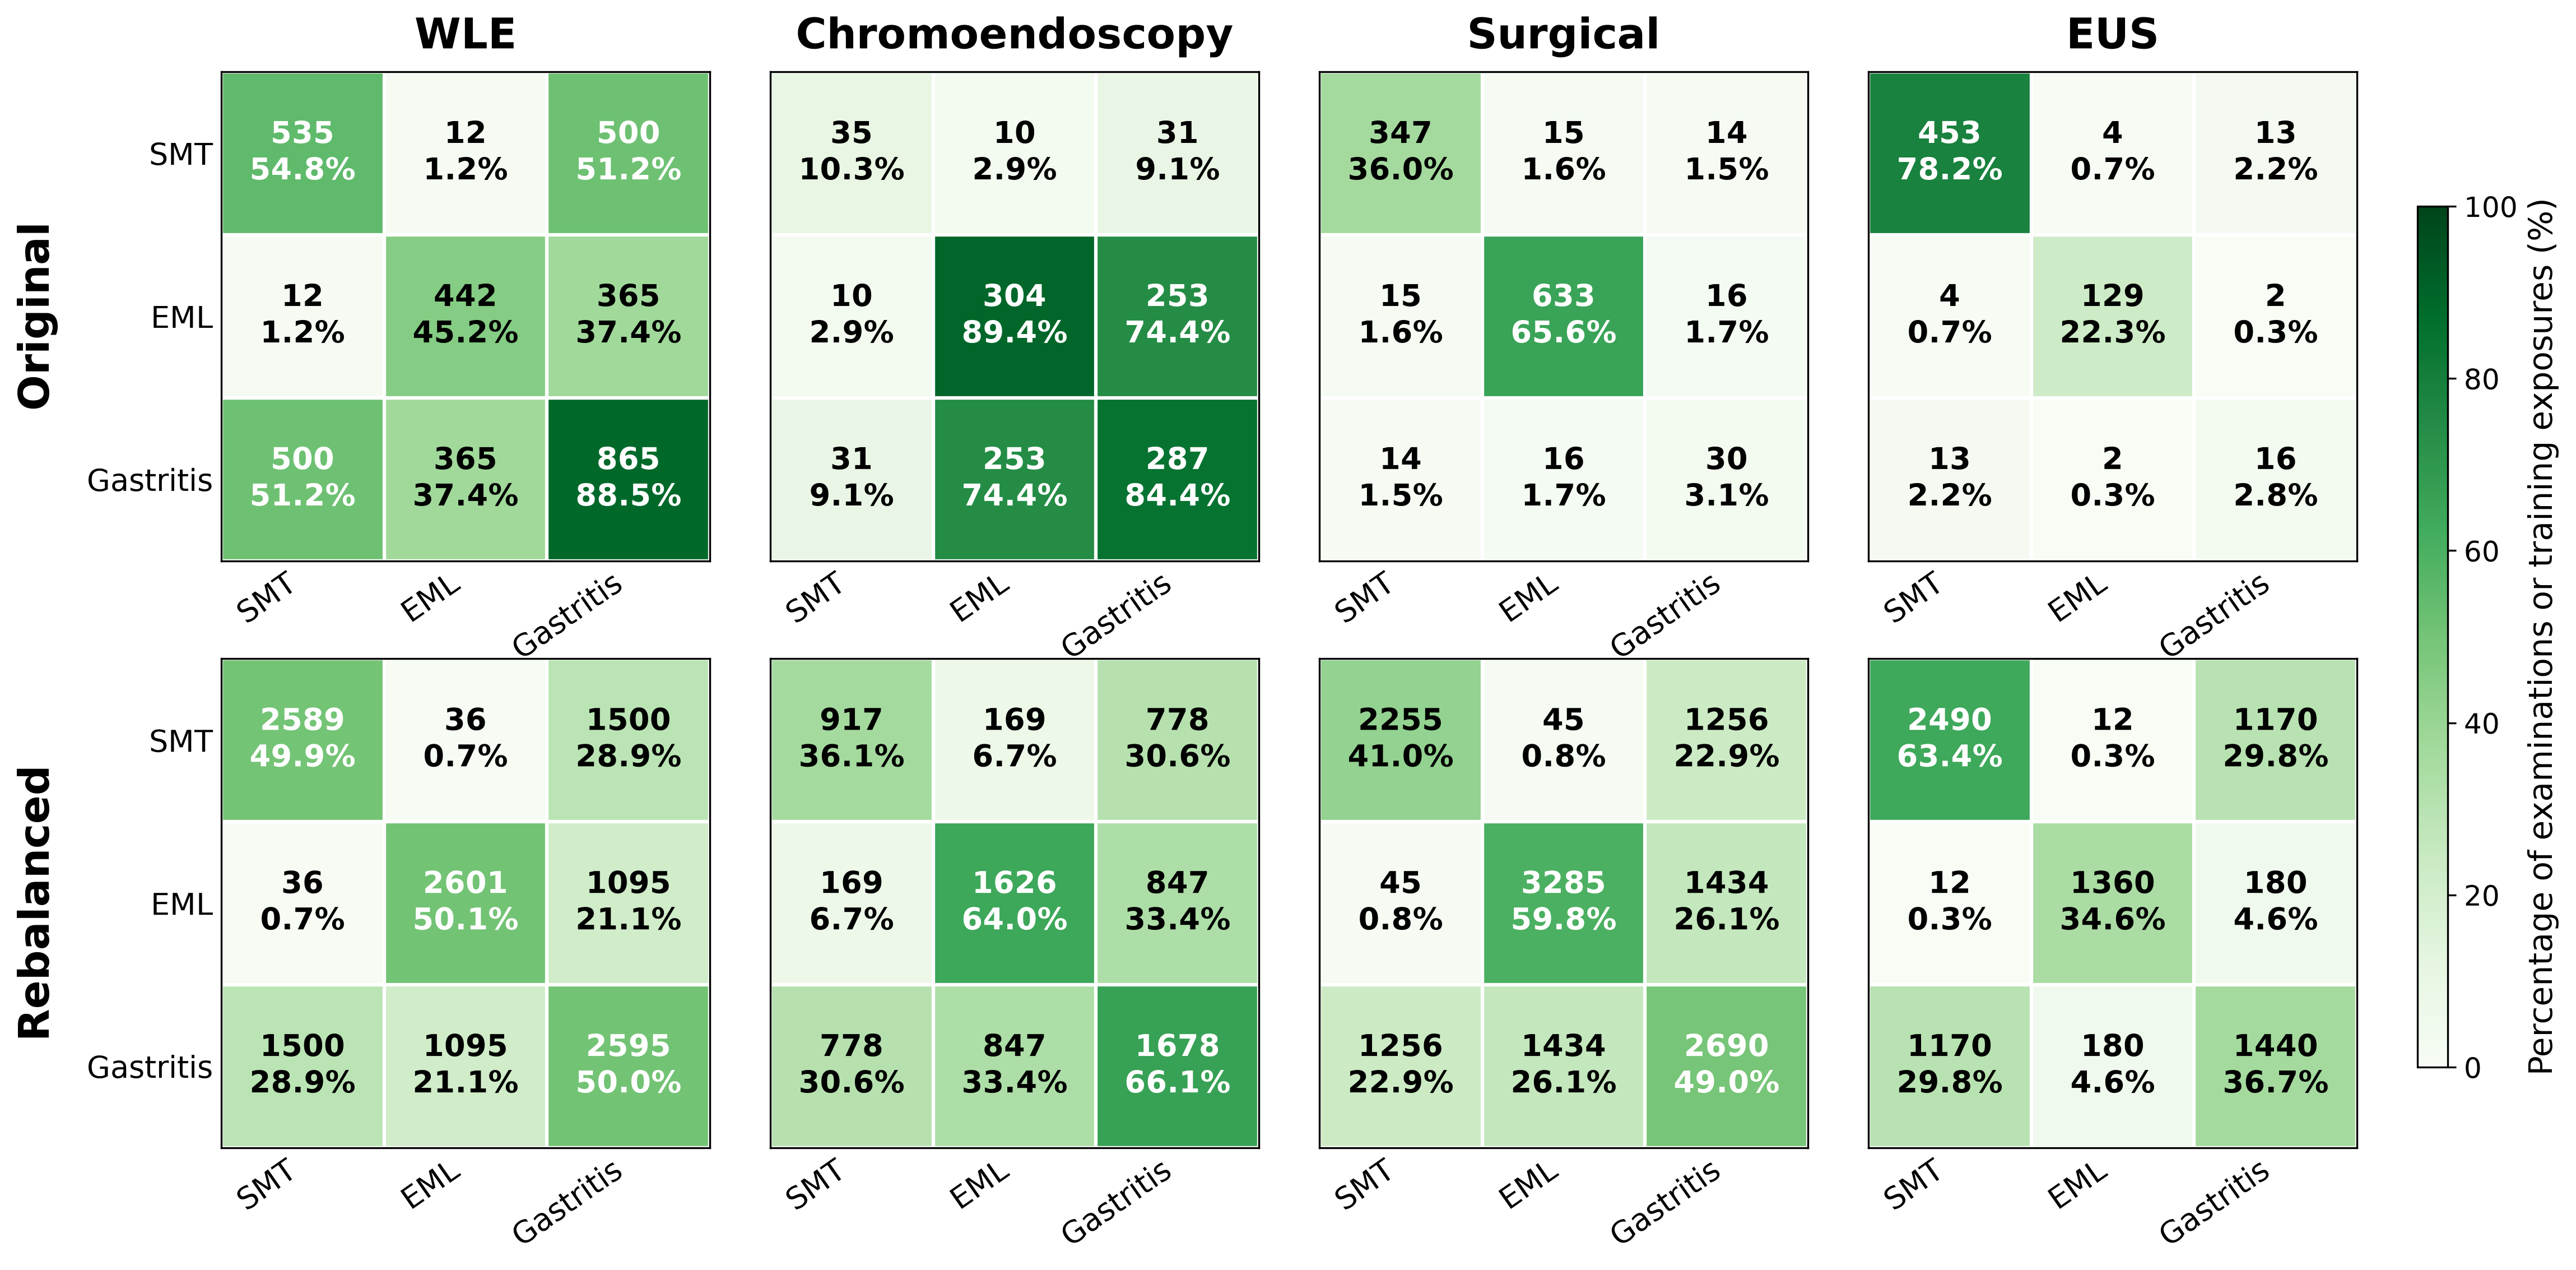
\includegraphics[width=\textwidth]{figs/label_cooccurrence_overview.png}
\caption{四个胃镜数据集的原始与重平衡标签共现矩阵。各列依次展示WLE、染色胃镜、手术胃镜和EUS的分布。上排为原始检查分布，下排为每个数据集中五个独立重平衡训练集汇总后的累积分布；验证集和测试集均未重平衡，也未纳入汇总。每个单元格给出相应数量和百分比。对角线表示单标签阳性频率，非对角线表示两两共阳性频率。百分比以对应原始数据集或汇总训练曝光为基数计算。SMT表示食管黏膜下肿瘤，EML表示食管黏膜病变。\label{fig:label_cooccurrence}}
\end{figure*}

\subsubsection{检查级多模态样本构建}

每次符合条件的检查由完整有序图像序列、三维多标签目标和胃镜所见描述文本表示。模型准备阶段从每次检查中最多均匀采样$T=64$张图像，并保持其原始顺序。每张图像被缩放至224$\times$224像素。二值掩码$M_i=\{m_{i1},\ldots,m_{iT}\}$用于区分有效图像和填充位置。与检查匹配的胃镜所见描述文本作为文本输入，其类别掩码和编码过程将在文本编码部分中说明。

\subsection{AMEF-MIL总体结构}

如图~\ref{fig:model_architecture}所示，AMEF-MIL将每次检查组织为有序图像bag、有效图像掩码、所见描述和检查级多标签目标。图像分支通过共享ConvNeXt-Tiny骨干网络和投影层提取实例特征。APro-CoPE保留原始采集坐标，构建内容自适应上下文坐标，并向双向Transformer传递绝对与相对位置关系。多标签注意力MIL进一步生成疾病特异性视觉表征，标签超图推理器通过共存发现之间的高阶交互对其进行细化。文本分支通过类别名称掩码和多尺度TextCNN将所见描述编码为token级特征。每个经过细化的视觉标签表征通过标签查询cross-attention检索疾病相关文本证据，门控残差模块再将检索表征与对应视觉表征进行融合。融合表征驱动主要多模态分支，超图细化后的视觉表征驱动辅助纯图像分支。训练阶段的真实标签监督共同优化两个分支，预训练多模态教师则向纯图像分支提供预测级知识。图~\ref{fig:apro_cope}进一步展示APro-CoPE的数学构造。

\begin{figure*}[t]
\centering
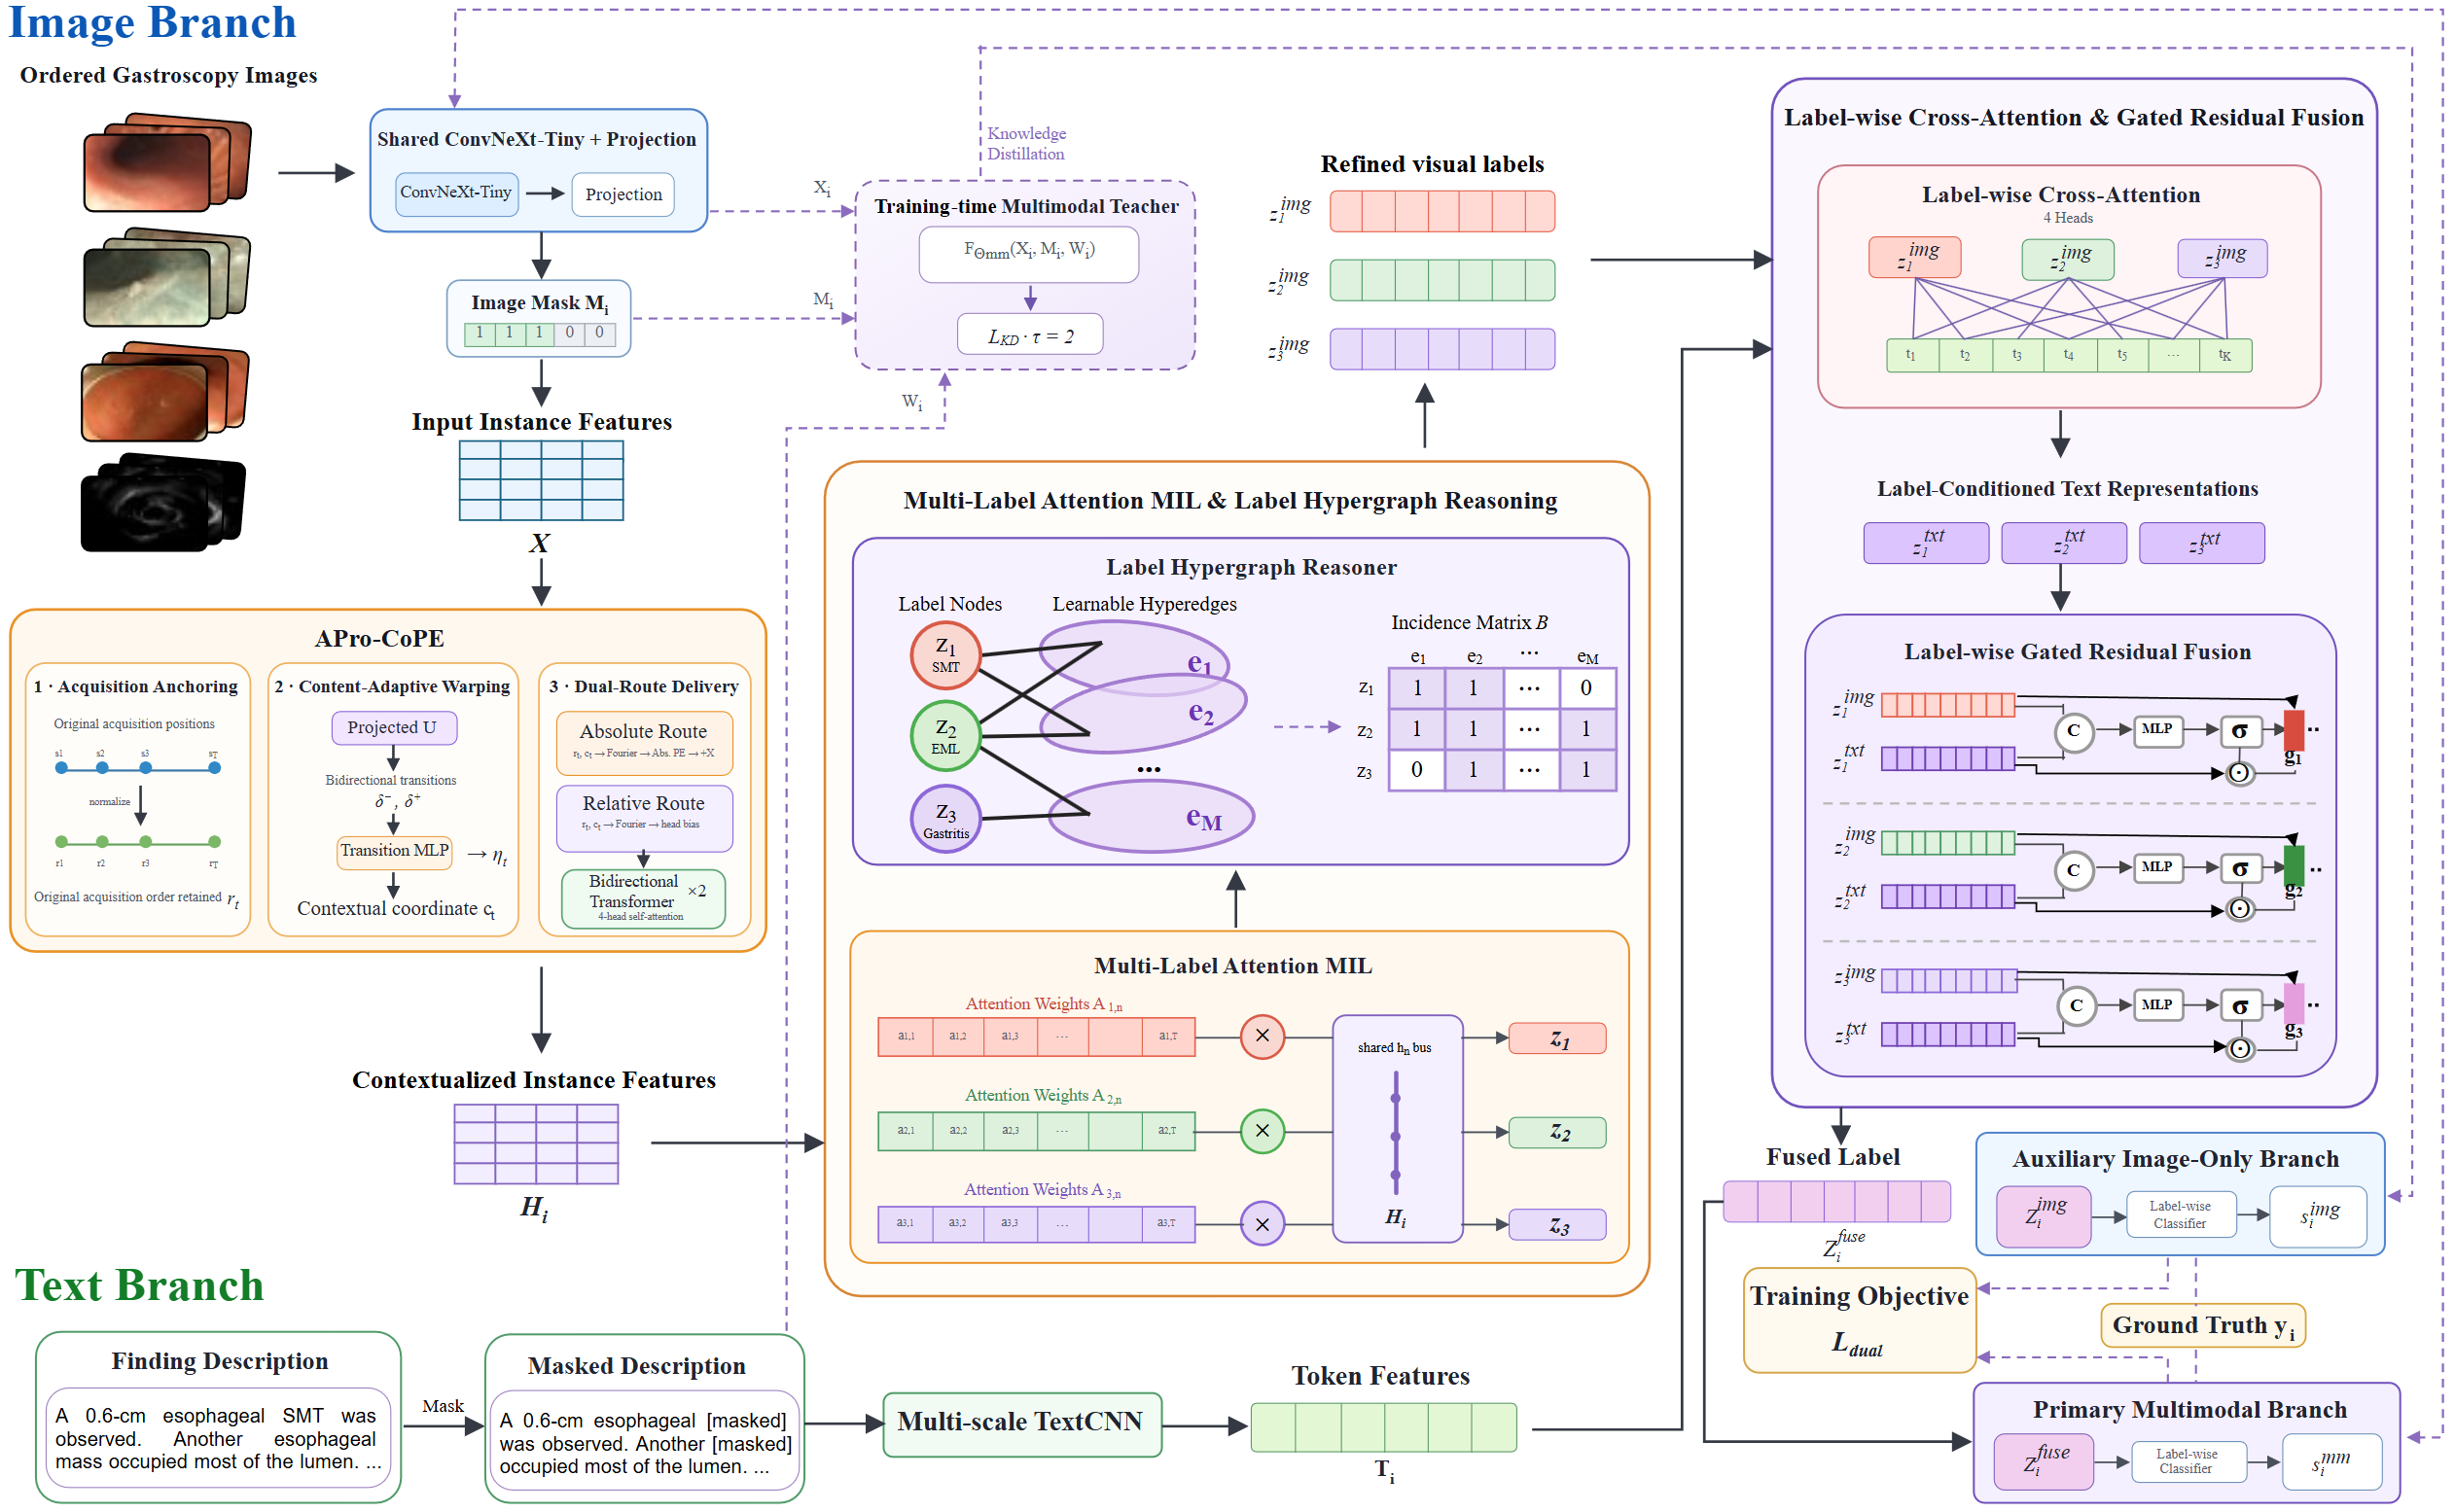
\includegraphics[width=\textwidth]{figs/amef_mil_overall_architecture.png}
\caption{AMEF-MIL总体结构。图像分支结合共享视觉编码、基于APro-CoPE的双向上下文建模、多标签注意力MIL和标签超图推理。文本分支采用多尺度TextCNN编码经过类别名称掩码的所见描述。标签级交叉注意力和门控残差融合生成主要多模态预测；经超图细化的视觉表征支持辅助纯图像预测，并在训练阶段接收来自预训练多模态教师的知识。\label{fig:model_architecture}}
\end{figure*}

\subsection{图像编码}

对于第$i$次胃镜检查，令$X_i=\{I_{i1},I_{i2},\ldots,I_{iN_i}\}$表示变长图像bag，$M_i$表示有效图像掩码，$y_i\in\{0,1\}^{L}$表示检查级目标，其中$L=3$。三个维度分别对应食管黏膜下肿瘤、食管粘膜病变和胃炎，同一次检查可以同时具有多个阳性标签。图像编码器根据$X_i$和$M_i$生成标签特异性视觉表征，随后由两个预测分支共同使用。

\subsubsection{图像编码与APro-CoPE流程上下文建模}

每张采样图像由共享的ConvNeXt-Tiny骨干网络和投影头进行编码，得到$d=512$维实例特征$x_{it}$。相比于传统的基于采样槽位编号的位置编码，本文提出更具创新性的采集锚定式流程上下文位置编码APro-CoPE。该方法受CoPE上下文相关位置递增思想启发，但针对非因果临床采集序列重新设计，引入显式采集锚点、单调性约束和端点守恒。图~\ref{fig:apro_cope}概括了采集坐标锚定、上下文坐标构造以及双路径位置注入过程。 \cite{R28}

设$s_{it}\in\{0,\ldots,N_i-1\}$为第$t$张采样图像在包含$N_i$张原始图像的完整检查中的索引，其原始采集锚点定义为
\begin{equation}
r_{it}=\frac{s_{it}}{\max(N_i-1,1)}.
\end{equation}
因此，无论采用均匀还是非均匀采样，原始流程坐标都不会被采样后的槽位坐标替代。首先将视觉特征投影为$u_{it}=\operatorname{LN}(W_px_{it})$，并构造后向转变$\delta^-_{it}=u_{it}-u_{i,t-1}$和前向转变$\delta^+_{it}=u_{i,t+1}-u_{it}$。随后根据当前特征、两个有符号转变、转变幅度、二者的逐元素一致性以及原始采集间隔估计持续转变分数：
\begin{equation}
\begin{aligned}
\eta_{it}={}&\alpha\tanh\!\Bigl(\operatorname{MLP}\!\bigl(
[u_{it},\delta^-_{it},\delta^+_{it},\\
&|\delta^-_{it}|,|\delta^+_{it}|,
\delta^-_{it}\odot\delta^+_{it},\Delta r_{it}]\bigr)\Bigr),
\end{aligned}
\end{equation}
其中$\Delta r_{it}=r_{it}-r_{i,t-1}$，$\alpha=1.5$用于限制坐标变形幅度。上下文间隔与上下文坐标定义为
\begin{align}
g_{it}&=\Delta r_{it}\exp(\eta_{it}),\\
\widetilde g_{it}&=\frac{(r_{iT_i}-r_{i1})g_{it}}{\sum_{k=2}^{T_i}g_{ik}},\\
c_{i1}&=r_{i1},\qquad c_{it}=r_{i1}+\sum_{k=2}^{t}\widetilde g_{ik},
\end{align}
其中$T_i$为有效采样图像数。由于变形后的每个间隔均为正值，且所有间隔会重新归一化到实际采集跨度，$c_{it}$保持单调，并保留序列的起点和终点。

APro-CoPE通过两条互补路径提供位置信息。绝对位置路径将
\begin{equation}
\begin{aligned}
p^{\mathrm{abs}}_{it}={}&f_{\mathrm{abs}}([\phi(r_{it}),\phi(c_{it}),\\
&\phi(c_{it}-r_{it})])
\end{aligned}
\end{equation}
加入$x_{it}$，其中$\phi(\cdot)$表示包含8个频率的连续Fourier映射。相对位置路径生成注意力头特异的偏置
\begin{equation}
\begin{aligned}
b^{(h)}_{itu}={}&2\tanh f^{(h)}_{\mathrm{rel}}\bigl([\phi(r_{it}-r_{iu}),
\phi(c_{it}-c_{iu}),\\
&\phi((c_{it}-c_{iu})-(r_{it}-r_{iu}))]\bigr).
\end{aligned}
\end{equation}
最终特征输入包含两层和四个注意力头的双向Transformer，并将$b^{(h)}_{itu}$加入缩放点积注意力logit。有效图像掩码在整个计算过程中排除填充位置，输出$H_i=\{h_{i1},\ldots,h_{iT_i}\}\in\mathbb{R}^{T_i\times d}$。

\begin{figure*}[t]
\centering
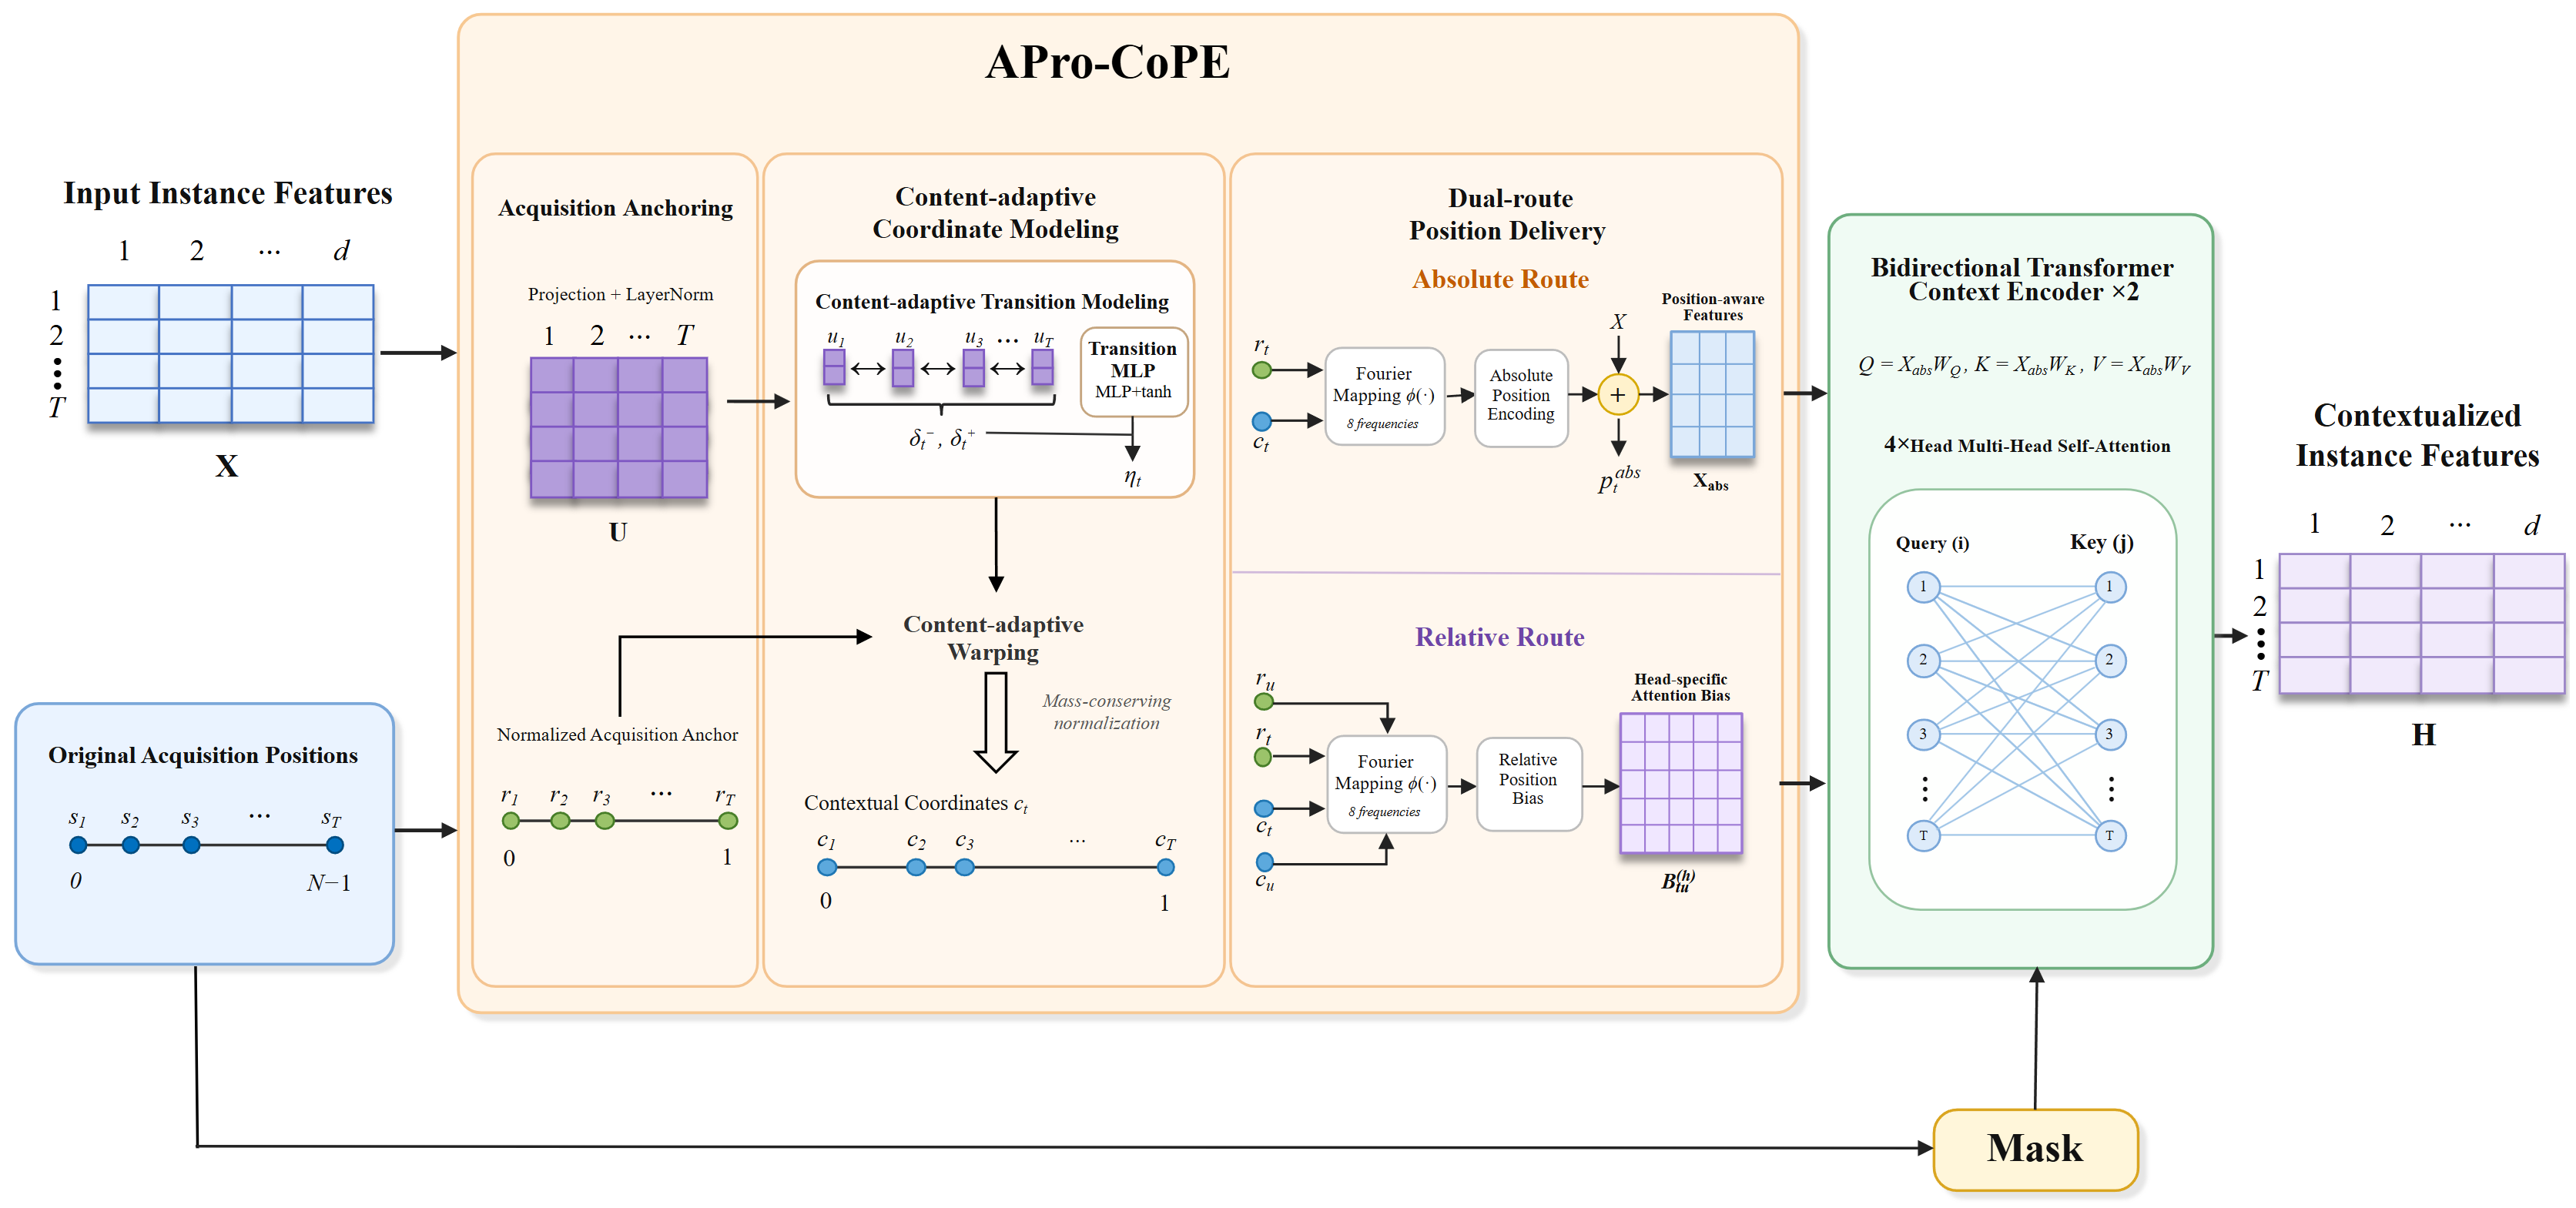
\includegraphics[width=\textwidth]{figs/apro_cope_bidirectional_transformer.png}
\caption{APro-CoPE结构。原始采集索引用于定义归一化采集锚点；双向视觉转变用于估计有界上下文变形分数；质量守恒归一化在保留观测序列端点的同时构建单调上下文坐标。绝对位置路径增强实例特征，相对位置路径向双向Transformer提供注意力头特异性偏置。\label{fig:apro_cope}}
\end{figure*}

\subsubsection{多标签注意力MIL}

同一次检查中的不同疾病可能由不同图像提供证据，因此模型为每个标签分别学习门控注意力分布。对于图像$n$，共享门控注意力特征为
\begin{equation}
q_{in}=\tanh(Vh_{in})\odot\sigma(Uh_{in}),
\end{equation}
标签$\ell$对应的注意力得分和归一化权重为
\begin{equation}
\begin{aligned}
e_{i\ell n}&=w_{\ell}^{\top}q_{in},\\
a_{i\ell n}&=\frac{m_{in}\exp(e_{i\ell n})}
{\sum_{t=1}^{T}m_{it}\exp(e_{i\ell t})+\epsilon}.
\end{aligned}
\end{equation}
标签特异性视觉表征计算为
\begin{equation}
z_{i\ell}=\sum_{n=1}^{T}a_{i\ell n}h_{in}.
\end{equation}
该操作使每种疾病能够聚合各自的支持图像，同时忽略无效位置。

\subsubsection{标签超图推理}

令$Z_i=[z_{i1},\ldots,z_{iL}]^{\top}\in\mathbb{R}^{L\times d}$表示标签特异性视觉特征矩阵。为建模多个共存疾病之间的高阶关系，标签超图推理器学习关联矩阵$B\in\mathbb{R}^{L\times E}$，其中$E=2$表示两个潜在超边。归一化后，信息先从标签节点传播到超边，再从超边返回标签节点：
\begin{equation}
U_i=S_{node\rightarrow edge}^{\top}\eta(Z_i),
\end{equation}
\begin{equation}
\widetilde{Z}_i=S_{edge\rightarrow node}U_i,
\end{equation}
\begin{equation}
Z_i^{img}=Z_i+\phi([Z_i;\widetilde{Z}_i]),
\end{equation}
其中$\eta(\cdot)$和$\phi(\cdot)$为可学习变换。所得$Z_i^{img}$为每种疾病保留一个经过超图细化的视觉表征，并作为两个预测分支共同使用的视觉输入。

\subsection{文本编码}

\subsubsection{所见描述选择与类别名称掩码}

文本编码器使用胃镜所见描述文本。该文本记录病灶形态、位置和周围黏膜改变，但也可能直接包含目标类别名称。为减少直接标签信息泄露，模型在分词前将与三个目标相关的标准疾病名称、缩写和直接词汇变体替换为统一掩码token。掩码词典覆盖食管黏膜下肿瘤或SMT、食管粘膜病变以及不同命名形式的胃炎等直接类别表述，同时保留解剖位置和描述性形态信息。所有数据子集使用相同的掩码过程。

\subsubsection{基于TextCNN的所见描述编码}

完成类别名称掩码后，首先规范化文本中的空格和标点，并将每份胃镜所见描述$W_i$切分为中文字符和字母数字片段。所得token以确定性方式映射至大小为8192的固定词表，并转换为128维嵌入。所见描述的最大长度设为$K=128$，超长序列被截断，较短序列使用填充补齐，同时采用二值文本掩码标记有效token位置。记嵌入后的token序列为$E_i\in\mathbb{R}^{K\times128}$，多尺度TextCNN使用卷积核大小$r\in\{2,3,4\}$的并行一维卷积，并通过等长填充保持序列长度：
\begin{equation}
H_i^{(r)}=\mathrm{ReLU}\!\left(\mathrm{Conv1D}_{r}(E_i)\right),
\qquad r\in\{2,3,4\}.
\end{equation}
随后，将不同尺度的卷积特征进行拼接、归一化，并投影至与视觉特征相同的$d=512$维空间：
\begin{equation}
\begin{aligned}
T_i={}&\mathrm{Dropout}\!\Bigl(\mathrm{GELU}\!\bigl(
W_t\,\mathrm{LN}\!\left([H_i^{(2)};H_i^{(3)};H_i^{(4)}]\right)\\
&\qquad+b_t\bigr)\Bigr)\in\mathbb{R}^{K\times d}.
\end{aligned}
\end{equation}
文本掩码用于抑制$T_i$中的填充位置，有效的token级表征被保留用于标签查询cross-attention。嵌入层、卷积层和投影层参数与完整模型联合优化。

\subsection{跨模态融合}

\subsubsection{标签查询交叉注意力与门控融合}

视觉表征与文本表征以不同粒度编码互补证据：$Z_i^{img}\in\mathbb{R}^{L\times d}$为每种疾病保留一个检查级表征，而$T_i\in\mathbb{R}^{K\times d}$保留所见描述中的token级信息。若直接将$T_i$池化为单一向量，所有标签将被迫共享同一文本摘要。因此，本文将经过超图细化的视觉标签表征$z_{i\ell}^{img}$作为query，将所见描述token作为key和value。对于注意力头$h\in\{1,\ldots,H\}$，其中$H=4$且$d_h=d/H$，query、key和value的投影分别为
\begin{equation}
\begin{aligned}
q_{i\ell}^{(h)}&=(z_{i\ell}^{img}+u_{\ell})W_Q^{(h)},\qquad
k_{ik}^{(h)}=t_{ik}W_K^{(h)},\\
v_{ik}^{(h)}&=t_{ik}W_V^{(h)},
\end{aligned}
\end{equation}
其中$u_{\ell}\in\mathbb{R}^{d}$为可学习的标签身份嵌入，用于在文本检索过程中保持不同疾病query之间的区分性。
令$\mu_{ik}\in\{0,1\}$表示第$k$个文本位置是否有效，标签到token的注意力得分和归一化权重计算为
\begin{equation}
\begin{aligned}
e_{i\ell k}^{(h)}&=\frac{q_{i\ell}^{(h)}{k_{ik}^{(h)}}^{\top}}{\sqrt{d_h}},\\
\alpha_{i\ell k}^{(h)}&=
\frac{\mu_{ik}\exp(e_{i\ell k}^{(h)})}
{\sum_{u=1}^{K}\mu_{iu}\exp(e_{i\ell u}^{(h)})+\epsilon}.
\end{aligned}
\end{equation}
由此，填充位置不参与文本检索，每个疾病标签则在同一份所见描述上分别学习独立的注意力分布。各注意力头的文本上下文以及最终的标签条件文本表征为
\begin{equation}
\begin{aligned}
o_{i\ell}^{(h)}&=\sum_{k=1}^{K}\alpha_{i\ell k}^{(h)}v_{ik}^{(h)},\\
z_{i\ell}^{txt}&=\operatorname{Concat}_{h=1}^{H}\!\left(o_{i\ell}^{(h)}\right)W_O.
\end{aligned}
\end{equation}
将所有标签的表征堆叠后得到$Z_i^{txt}\in\mathbb{R}^{L\times d}$。该设计在融合过程中保留标签对应关系，使标签$\ell$的视觉证据能够检索服务于同一预测的文本证据，而不是对所有标签不加区分地使用同一个所见描述表征。

考虑到不同疾病和不同检查中所检索文本的相关性与可靠性并不相同，模型为每个标签分别估计一个标量门控系数：
\begin{equation}
g_{i\ell}=a_i\,\sigma\!\left(\rho([z_{i\ell}^{img};z_{i\ell}^{txt}])\right),
\end{equation}
其中$\rho(\cdot)$为两层多层感知机，$a_i\in\{0,1\}$表示该次检查是否包含有效所见描述文本。融合表征通过门控残差注入得到：
\begin{equation}
z_{i\ell}^{fuse}=z_{i\ell}^{img}+g_{i\ell}z_{i\ell}^{txt}.
\end{equation}
残差形式保留原始视觉表征，同时允许模型根据具体检查和疾病标签，以自适应幅度引入相关语义证据。当不存在有效所见描述文本时，$a_i=0$，此时$z_{i\ell}^{fuse}=z_{i\ell}^{img}$。

为显式约束标签与文本之间的对应关系，本文进一步引入标签查询判别损失。对于阳性标签$\ell$和未出现的标签$r$，令$\widetilde{s}_{i\ell\leftarrow r}^{mm}$表示将$z_{i\ell}^{txt}$替换为$z_{ir}^{txt}$、同时保持标签$\ell$的视觉表征、门控和分类器不变时得到的反事实logit。有效比较集合定义为$\mathcal{P}_i=\{(\ell,r)\mid a_i=1,\ y_{i\ell}=1,\ y_{ir}=0,\ \ell\neq r\}$，相应损失为
\begin{equation}
\begin{aligned}
\mathcal{L}_{LQD}={}&-\frac{1}{\sum_i|\mathcal{P}_i|}
\sum_i\sum_{(\ell,r)\in\mathcal{P}_i}\Big[
\log\sigma(s_{i\ell}^{mm})\\
&+\log\left(1-\sigma(\widetilde{s}_{i\ell\leftarrow r}^{mm})\right)\Big].
\end{aligned}
\end{equation}
该损失促使正确标签query检索的文本支持其阳性疾病预测，同时抑制未出现疾病query所检索的文本成为可互换证据。共存的阳性标签对不参与该约束，以保留临床上有效的疾病共存信息。

\subsection{预测分支}

\subsubsection{主要多模态分支}

令$Z_i^{fuse}=[z_{i1}^{fuse},\ldots,z_{iL}^{fuse}]^{\top}$表示标签级融合表征。主要多模态分支将标签级分类器作用于该表征：
\begin{equation}
s_i^{mm}=C_{mm}(Z_i^{fuse}).
\end{equation}
该分支参数与共享图像编码器、文本编码器及跨模态融合模块共同使用检查级非对称损失进行优化：
\begin{equation}
\mathcal{L}_{mm}=\mathcal{L}_{ASL}(s_i^{mm},y_i)+\lambda_q\mathcal{L}_{LQD}.
\end{equation}
其中$\lambda_q$用于控制标签查询判别约束的权重。
该分支构成主要预测路径，同时使用内镜图像序列和经过类别名称掩码的胃镜所见描述。

为向纯图像分支迁移知识，首先使用$\mathcal{L}_{mm}$预训练具有相同路径的多模态模型，随后固定所选模型参数，并记为$\overline{\Theta}_{mm}$。对于同一次检查，冻结教师生成logits：
\begin{equation}
\overline{s}_i^{mm}=F_{\overline{\Theta}_{mm}}(X_i,M_i,W_i),
\end{equation}
其中$W_i$表示经过类别名称掩码的所见描述文本。冻结教师仅提供软目标，在后续纯图像训练过程中不接收梯度。

\subsubsection{纯图像分支与多模态知识迁移}

辅助纯图像分支直接根据经过超图细化的视觉表征进行预测：
\begin{equation}
s_i^{img}=C_{img}(Z_i^{img}).
\end{equation}
该分支使用相同的检查级目标进行基础监督：
\begin{equation}
\mathcal{L}_{img}=\mathcal{L}_{ASL}(s_i^{img},y_i).
\end{equation}
当可训练的多模态分支接受联合监督时，$\mathcal{L}_{mm}$还会更新共享视觉编码器，从而为纯图像路径提供间接的表征级学习信号。

知识蒸馏则由冻结的多模态教师提供独立的预测级迁移信号。温度为$\tau$时，教师概率和多标签蒸馏损失分别定义为
\begin{equation}
\overline{p}_i^{mm}=\sigma\!\left(\frac{\overline{s}_i^{mm}}{\tau}\right),
\end{equation}
\begin{equation}
\begin{aligned}
\mathcal{L}_{KD}={}&\tau^2\operatorname{BCEWithLogits}\!\left(
\frac{s_i^{img}}{\tau},\right.\\
&\left.\operatorname{sg}(\overline{p}_i^{mm})\right),
\end{aligned}
\end{equation}
其中$\operatorname{sg}(\cdot)$表示教师目标不参与梯度反向传播。联合训练目标写为
\begin{equation}
\begin{aligned}
\mathcal{L}_{dual}={}&\mathcal{L}_{img}+\lambda_{mm}\mathcal{L}_{mm}\\
&+\lambda_{KD}\mathcal{L}_{KD},
\end{aligned}
\end{equation}
其中$\lambda_{mm}$和$\lambda_{KD}$分别控制多模态分支监督与冻结教师蒸馏的贡献。纯图像推理时只需要$X_i$、$M_i$和$C_{img}$，不使用所见描述编码器、跨模态融合模块或冻结教师。

\section{实验}

\subsection{实验设置}

所有实验均采用前文所述的患者分组五折协议，并使用随机种子2026。模型采用AdamW训练最多30个epoch，初始学习率为$2\times10^{-5}$，权重衰减为0.02，检查级batch size为1，并对连续4次检查累积梯度。前20\%优化步采用线性学习率预热，随后使用余弦衰减。训练过程中启用自动混合精度，dropout设为0.2，多标签监督采用非对称损失。所有实验以折为单位，在6张NVIDIA GeForce RTX 4090 GPU上独立运行。

图像端将输入图像缩放至224$\times$224像素，并采用冻结第一阶段的预训练ConvNeXt-Tiny进行编码。除另有说明外，每次检查均匀采样最多64张图像，投影后的特征维度为512。上下文编码器包含2层双向Transformer和4个注意力头，标签超图包含2个潜在超边。完整APro-CoPE采用64维转变空间、8个Fourier频率、$\alpha=1.5$、质量守恒以及绝对与相对双位置路由。文本端将所见描述长度限制为128个token，采用大小为8192的词表、128维嵌入以及卷积核大小为2、3和4的TextCNN进行编码。标签查询cross-attention包含4个注意力头，随后进行标签级门控残差融合，标签查询判别损失的权重设为$\lambda_q=0.01$。主要多模态输出同时使用内镜图像序列和经过类别名称掩码的胃镜所见描述。在纯图像迁移实验中，辅助纯图像分类损失的权重设为0.5，蒸馏损失权重设为0或1，温度为$\tau=2$。

本文采用宏平均F1作为主要评价指标和模型选择指标，因为在类别不平衡条件下，该指标对三个目标标签赋予相同权重。每折选择验证集宏平均F1最高的检查点，最终结果报告患者分组五折的均值和标准差。所有实验比较均已通过统计显著性检验。

\subsection{总体性能比较与标签级分析}

\subsubsection{纯图像、纯文本与多模态模型比较}

为评价检查级分类的总体性能，本文在相同的患者分组五折协议下，将AMEF-MIL与纯图像MIL方法、纯文本编码器和多模态分类模型进行比较。对于4种多模态对比方法，本文将其融合机制适配至检查级图像bag与经过类别名称掩码的胃镜所见描述，同时保持统一的数据划分和优化设置。\cite{R29,R30,R31,R32}

表~\ref{T2}给出了比较结果。AMEF-MIL在四个数据集上均取得最高的平均宏平均F1：WLE为0.9149、染色胃镜为0.8877、手术胃镜为0.8456、EUS为0.9064。在每个数据集上，AMEF-MIL均优于表现最好的纯图像模型和纯文本模型。这一结果直接表明，模型能够整合有序图像序列与经过类别名称掩码的胃镜所见描述各自提供的判别信息，形成有效的跨模态互补表征，体现了AMEF-MIL的多模态建模能力。AMEF-MIL在四个数据集上还均优于所选多模态基线，说明由采集感知图像编码、标签超图推理、疾病特异性cross-attention和门控残差融合构成的完整pipeline更适合检查级多标签分类任务。其中，染色胃镜上的优势最为突出，AMEF-MIL同时取得全部对比方法中最高的平均宏平均F1和最小的折间标准差。

\begin{table*}[t]
\scriptsize\tabletimes\centering
\caption{四个胃镜数据集上纯图像、纯文本与多模态方法的比较。数值为患者分组五折宏平均F1的均值$\pm$标准差。img.和txt.分别表示内镜图像输入和经过类别名称掩码的胃镜所见描述输入。\label{T2}}
\resizebox{\textwidth}{!}{%
\begin{tabular}{lcc*{4}{c}}
\hline
模型 & 图像 & 文本 & WLE & 染色胃镜 & 手术胃镜 & EUS \\
\hline
Attention MIL & $\checkmark$ & $\times$ & \tresult{0.7919}{0.0119} & \tresult{0.7391}{0.0448} & \tresult{0.7018}{0.1235} & \tresult{0.6268}{0.0342} \\
Mean pooling & $\checkmark$ & $\times$ & \tresult{0.7931}{0.0088} & \tresult{0.7408}{0.0322} & \tresult{0.7173}{0.0744} & \tresult{0.5910}{0.0592} \\
Transformer-context MIL & $\checkmark$ & $\times$ & \tresult{0.8004}{0.0160} & \tresult{0.7426}{0.0194} & \tresult{0.7765}{0.0886} & \tresult{0.5966}{0.0612} \\
Top-$k$ MIL & $\checkmark$ & $\times$ & \tresult{0.7862}{0.0232} & \tresult{0.7511}{0.0406} & \tresult{0.7698}{0.0849} & \tresult{0.6037}{0.0887} \\
Max pooling & $\checkmark$ & $\times$ & \tresult{0.7608}{0.0034} & \tresult{0.6842}{0.0261} & \tresult{0.6009}{0.0919} & \tresult{0.5505}{0.0756} \\
TransMIL & $\checkmark$ & $\times$ & \tresult{0.8021}{0.0146} & \tresult{0.7217}{0.0368} & \tresult{0.7516}{0.0938} & \tresult{0.6045}{0.0539} \\
DSMIL & $\checkmark$ & $\times$ & \tresult{0.7956}{0.0159} & \tresult{0.7468}{0.0448} & \tresult{0.6873}{0.0852} & \tresult{0.5765}{0.0765} \\
DTFD-MIL & $\checkmark$ & $\times$ & \tresult{0.7714}{0.0141} & \tresult{0.7091}{0.0306} & \tresult{0.7134}{0.0853} & \tresult{0.5896}{0.0419} \\
CLAM-MB & $\checkmark$ & $\times$ & \tresult{0.7741}{0.0090} & \tresult{0.7137}{0.0269} & \tresult{0.7094}{0.0865} & \tresult{0.5883}{0.0401} \\
CLAM-SB & $\checkmark$ & $\times$ & \tresult{0.7642}{0.0040} & \tresult{0.6997}{0.0234} & \tresult{0.6785}{0.0479} & \tresult{0.5695}{0.0379} \\
\hline
Hashed mean & $\times$ & $\checkmark$ & \tresult{0.8901}{0.0184} & \tresult{0.8037}{0.0689} & \tresult{0.8349}{0.0187} & \tresult{0.8836}{0.0688} \\
Vocabulary attention & $\times$ & $\checkmark$ & \tresult{0.8906}{0.0124} & \tresult{0.8045}{0.0708} & \tresult{0.8147}{0.0487} & \tresult{0.8957}{0.0542} \\
TextCNN & $\times$ & $\checkmark$ & \tresult{0.9004}{0.0123} & \tresult{0.8652}{0.0332} & \tresult{0.8356}{0.0807} & \tresult{0.8982}{0.0515} \\
BiGRU & $\times$ & $\checkmark$ & \tresult{0.8928}{0.0191} & \tresult{0.8085}{0.0818} & \tresult{0.8075}{0.0342} & \tresult{0.9019}{0.0531} \\
Transformer & $\times$ & $\checkmark$ & \tresult{0.8915}{0.0163} & \tresult{0.8150}{0.0281} & \tresult{0.8285}{0.0174} & \tresult{0.8830}{0.0604} \\
\hline
MMFNet (2024)\cite{R29}$^{\dagger}$ & $\checkmark$ & $\checkmark$ & \tresult{0.9132}{0.0099} & \tresult{0.8371}{0.0647} & \tresult{0.8345}{0.0844} & \tresult{0.8999}{0.0731} \\
RadFuse (2025)\cite{R32}$^{\dagger}$ & $\checkmark$ & $\checkmark$ & \tresult{0.9135}{0.0083} & \tresult{0.7990}{0.1013} & \tresult{0.8221}{0.0671} & \tresult{0.8517}{0.0712} \\
SAIF (2025)\cite{R30}$^{\dagger}$ & $\checkmark$ & $\checkmark$ & \tresult{0.8413}{0.0166} & \tresult{0.7201}{0.0544} & \tresult{0.7482}{0.0821} & \tresult{0.6266}{0.0986} \\
MMTF (2026)\cite{R31}$^{\dagger}$ & $\checkmark$ & $\checkmark$ & \tresult{0.9121}{0.0118} & \tresult{0.7320}{0.0415} & \tresult{0.7595}{0.1371} & \tresult{0.7846}{0.0974} \\
\hline
AMEF-MIL (Ours) & $\checkmark$ & $\checkmark$ & \tresult{\textbf{0.9149}}{\textbf{0.0114}} & \tresult{\textbf{0.8877}}{\textbf{0.0168}} & \tresult{\textbf{0.8456}}{\textbf{0.0224}} & \tresult{\textbf{0.9064}}{\textbf{0.0474}} \\
\hline
\end{tabular}
}
\par\raggedright\scriptsize $^{\dagger}$Reimplemented using the same examination-level inputs, category-masking procedure, patient-grouped folds, and optimization protocol as AMEF-MIL.
\end{table*}

\subsubsection{折外标签级混淆分析}

图~\ref{fig:oof_confusion_selected}通过汇总五个互斥测试折的预测进一步分析标签级判定，使每次符合条件的检查恰好参与一次折外评价。由于同一次检查可以具有多个阳性标签，本文分别报告一对其余$2\times2$混淆矩阵。

多数“数据集--标签”组合具有较高的阳性类别敏感度，包括WLE中食管黏膜下肿瘤的97.9\%和胃炎的97.7\%、染色胃镜中食管黏膜病变的99.0\%、手术胃镜中食管黏膜下肿瘤的94.5\%，以及EUS中食管黏膜下肿瘤的99.6\%。主要错误来自阴性检查相对较少标签的假阳性预测，其中染色胃镜中的食管黏膜病变和胃炎以及WLE中的胃炎较为明显。这些结果从标签层面补充了宏平均F1，并显示标签患病率和所选判定阈值如何影响敏感度与特异度之间的平衡。

\begin{figure*}[t]
\centering
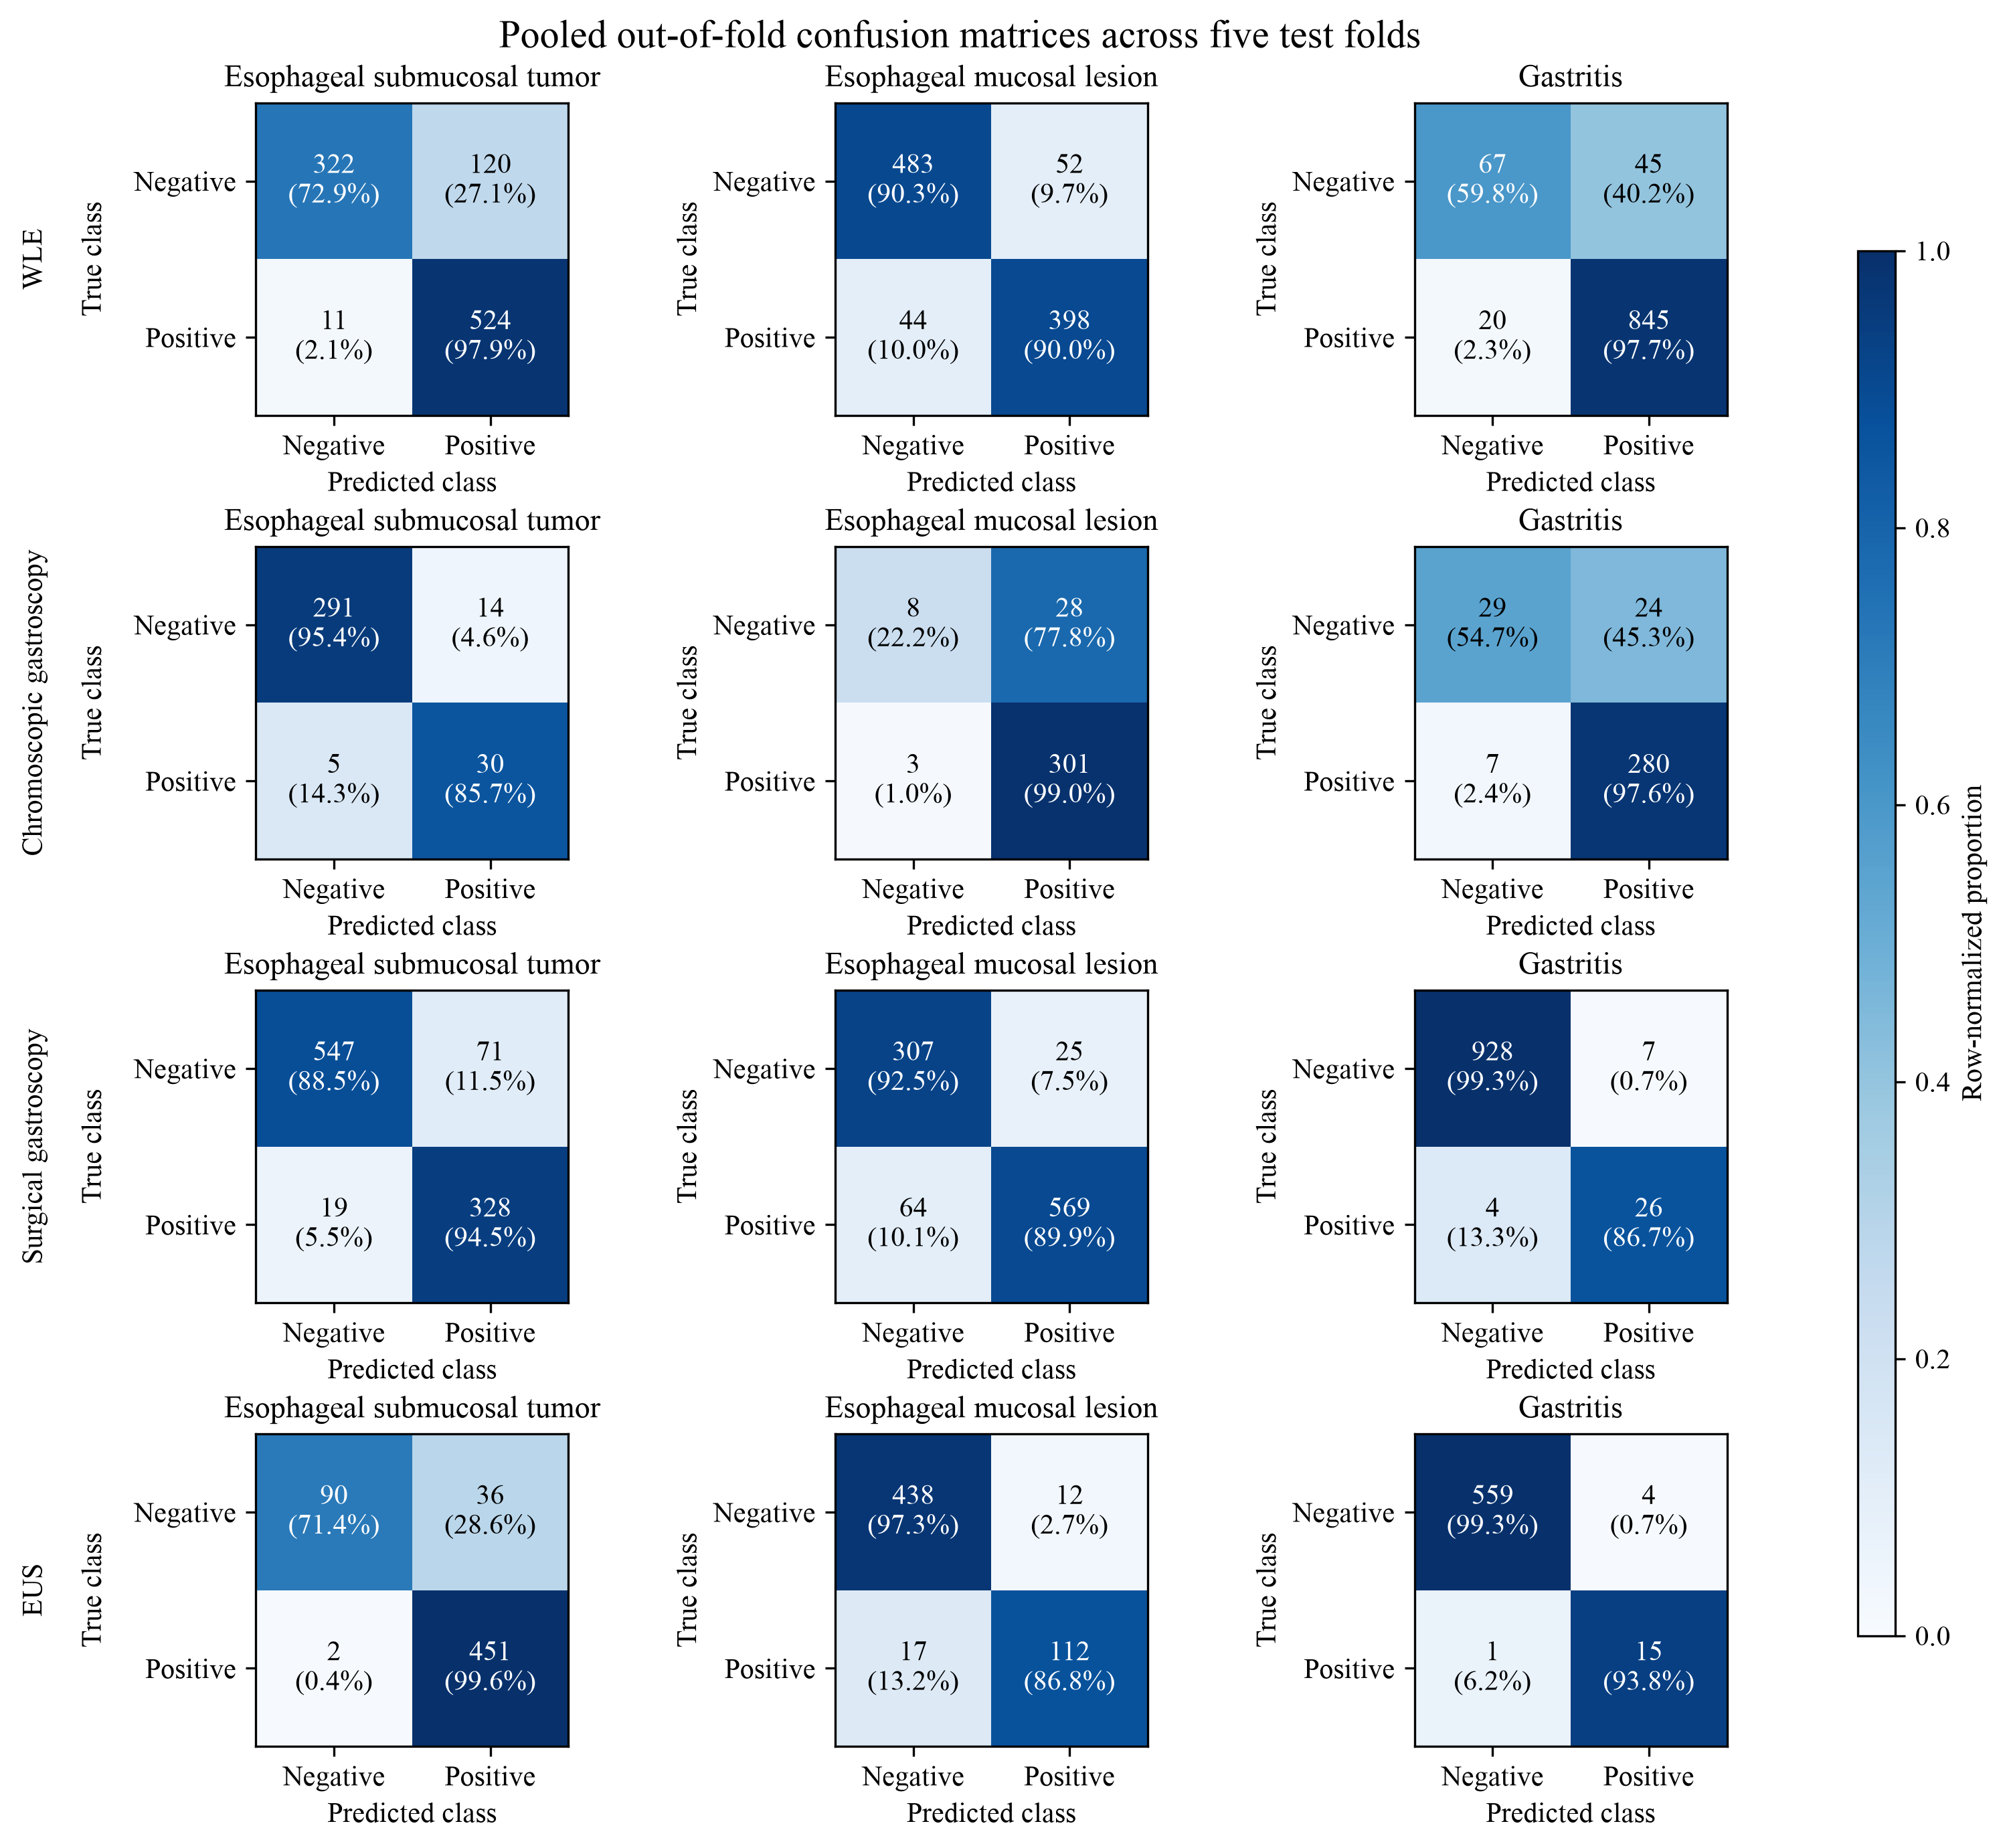
\includegraphics[width=\textwidth]{figs/selected_models_oof_confusion_matrices.png}
\caption{AMEF-MIL在五个患者分组测试折上汇总的折外一对其余混淆矩阵。各行依次对应WLE、染色胃镜、手术胃镜和EUS数据集，各列对应三个目标标签。每个单元格给出汇总数量和行归一化百分比，每次检查仅出现在一个测试折中。\label{fig:oof_confusion_selected}}
\end{figure*}

\subsection{模型组件分析与消融实验}

\subsubsection{图像预算与位置编码}

为分析增加采样图像数量能否使模型有效利用更大范围的检查信息，本文评估每次检查采样16、32、48、64、80和96张图像的6种图像预算。在每种图像预算下，本文比较不使用位置编码、使用采样槽位位置编码和使用APro-CoPE的相同上下文编码器，从而区分检查覆盖范围与位置建模各自带来的影响。

表~\ref{T3}的结果表明，在不使用位置编码时，增加图像数量所带来的增益逐渐减小，WLE在48张和80张图像时甚至出现局部性能下降。这说明，仅增加图像数量并不能保证上下文编码器有效利用扩展后的检查序列。加入采样槽位位置编码后，几乎所有匹配图像预算下的性能均得到改善，并且在染色胃镜、手术胃镜和EUS上随着图像数量增加呈现更稳定的提升。APro-CoPE在每组匹配的“数据集--图像预算”比较中均取得最高的平均宏平均F1，并且是唯一在四个数据集上均随图像数量从16张增加至96张而保持平均性能单调提升的配置。其中，染色胃镜上的提升尤为明显：APro-CoPE的宏平均F1由16张图像时的0.8134提高至64张图像时的0.8877，而不使用位置编码时相应结果仅由0.7478提高至0.7795。超过64张图像后，APro-CoPE在四个数据集上的额外增益仅为0.16--0.52个百分点，说明检查覆盖范围已接近实际性能饱和点。因此，后续消融实验统一采用64张图像，以在控制计算成本的同时保留大部分性能收益。

\begin{table*}[t]
\scriptsize\tabletimes\centering
\caption{四个胃镜数据集上采样图像预算与位置编码的影响。在每种图像预算下，使用相同上下文编码器分别评价无位置编码、采样槽位位置编码和APro-CoPE。数值为患者分组五折宏平均F1的均值$\pm$标准差。PE表示位置编码。\label{T3}}
\resizebox{\textwidth}{!}{%
\begin{tabular}{cl*{4}{c}}
\hline
图像数 & 方法 & WLE & 染色胃镜 & 手术胃镜 & EUS \\
\hline
16 & No PE & \tresult{0.8673}{0.0115} & \tresult{0.7478}{0.0513} & \tresult{0.7824}{0.0837} & \tresult{0.8443}{0.0803} \\
 & Sampled-slot PE & \tresult{0.8819}{0.0132} & \tresult{0.7789}{0.0683} & \tresult{0.8012}{0.0919} & \tresult{0.8712}{0.0663} \\
 & APro-CoPE (Ours) & \tresult{\textbf{0.8986}}{\textbf{0.0131}} & \tresult{\textbf{0.8134}}{\textbf{0.0368}} & \tresult{\textbf{0.8168}}{\textbf{0.0235}} & \tresult{\textbf{0.8879}}{\textbf{0.0635}} \\
\hline
32 & No PE & \tresult{0.8743}{0.0078} & \tresult{0.7535}{0.0341} & \tresult{0.7891}{0.0676} & \tresult{0.8537}{0.0758} \\
 & Sampled-slot PE & \tresult{0.8840}{0.0141} & \tresult{0.7978}{0.0794} & \tresult{0.8125}{0.0679} & \tresult{0.8836}{0.0749} \\
 & APro-CoPE (Ours) & \tresult{\textbf{0.9068}}{\textbf{0.0133}} & \tresult{\textbf{0.8460}}{\textbf{0.0297}} & \tresult{\textbf{0.8304}}{\textbf{0.0215}} & \tresult{\textbf{0.8979}}{\textbf{0.0564}} \\
\hline
48 & No PE & \tresult{0.8720}{0.0092} & \tresult{0.7635}{0.0438} & \tresult{0.7898}{0.0762} & \tresult{0.8594}{0.0926} \\
 & Sampled-slot PE & \tresult{0.8872}{0.0148} & \tresult{0.8249}{0.0690} & \tresult{0.8221}{0.0865} & \tresult{0.8915}{0.0672} \\
 & APro-CoPE (Ours) & \tresult{\textbf{0.9119}}{\textbf{0.0142}} & \tresult{\textbf{0.8732}}{\textbf{0.0240}} & \tresult{\textbf{0.8408}}{\textbf{0.0185}} & \tresult{\textbf{0.9030}}{\textbf{0.0434}} \\
\hline
64 & No PE & \tresult{0.8816}{0.0086} & \tresult{0.7795}{0.0351} & \tresult{0.8024}{0.0882} & \tresult{0.8694}{0.0974} \\
 & Sampled-slot PE & \tresult{0.8979}{0.0140} & \tresult{0.8592}{0.0761} & \tresult{0.8243}{0.0418} & \tresult{0.8999}{0.0617} \\
 & APro-CoPE (Ours) & \tresult{\textbf{0.9149}}{\textbf{0.0114}} & \tresult{\textbf{0.8877}}{\textbf{0.0168}} & \tresult{\textbf{0.8456}}{\textbf{0.0224}} & \tresult{\textbf{0.9064}}{\textbf{0.0474}} \\
\hline
80 & No PE & \tresult{0.8814}{0.0076} & \tresult{0.7818}{0.0426} & \tresult{0.8041}{0.0864} & \tresult{0.8715}{0.1026} \\
 & Sampled-slot PE & \tresult{0.8864}{0.0106} & \tresult{0.8665}{0.0508} & \tresult{0.8312}{0.0369} & \tresult{0.9021}{0.0598} \\
 & APro-CoPE (Ours) & \tresult{\textbf{0.9158}}{\textbf{0.0102}} & \tresult{\textbf{0.8906}}{\textbf{0.0214}} & \tresult{\textbf{0.8480}}{\textbf{0.0178}} & \tresult{\textbf{0.9089}}{\textbf{0.0452}} \\
\hline
96 & No PE & \tresult{0.8836}{0.0091} & \tresult{0.7856}{0.0397} & \tresult{0.8068}{0.0828} & \tresult{0.8731}{0.1034} \\
 & Sampled-slot PE & \tresult{0.8930}{0.0117} & \tresult{0.8706}{0.0658} & \tresult{0.8345}{0.0410} & \tresult{0.9042}{0.0635} \\
 & APro-CoPE (Ours) & \tresult{\textbf{0.9165}}{\textbf{0.0090}} & \tresult{\textbf{0.8929}}{\textbf{0.0177}} & \tresult{\textbf{0.8495}}{\textbf{0.0197}} & \tresult{\textbf{0.9103}}{\textbf{0.0442}} \\
\hline
\end{tabular}
}
\end{table*}

\subsubsection{APro-CoPE组件分析}

为确定APro-CoPE中不同设计的作用，本文将图像预算固定为64张，并在所有配置中使用相同的两层双向Transformer，仅改变位置机制。对比配置包括不使用位置编码的Transformer、采样槽位位置编码、双向CoPE、采集锚点位置编码以及APro-CoPE的组件级变体。

表~\ref{T3_apro}的结果表明，完整APro-CoPE在四个数据集上均取得最高的平均宏平均F1。与采样槽位位置编码相比，其在WLE、染色胃镜、手术胃镜和EUS上分别提高1.70、2.85、2.13和0.65个百分点。将持续转变机制替换为成对转变后，四个数据集的性能均有所下降，其中染色胃镜的下降最明显。移除质量守恒导致0.28--3.25个百分点的下降。仅保留绝对位置路径同样降低性能，而仅保留相对位置路径分别导致0.84、11.66、8.10和7.77个百分点的更大下降。仅使用采集锚点位置编码无法达到完整方法的性能。综合来看，内容自适应转变估计、端点保持归一化和双路径位置注入能够在采集锚点基础上提供互补信息，其中绝对位置路径对于在不同检查场景中维持稳定性能尤为重要。

\begin{table*}[t]
\footnotesize\tabletimes\centering
\caption{四个胃镜数据集上APro-CoPE的组件分析，每次检查采样64张图像。所有变体均采用相同的两层双向Transformer，仅改变位置机制。数值为患者分组五折宏平均F1的均值$\pm$标准差。w/o表示移除，PE表示位置编码，Trans.表示转变机制，CG表示内容门控，PW表示以成对转变替代PT，PT表示持续转变，AA表示采集锚点，MC表示质量守恒，Abs.表示绝对位置路径，Rel.表示相对位置路径。\label{T3_apro}}
\setlength{\tabcolsep}{3pt}
\resizebox{\textwidth}{!}{%
\begin{tabular}{@{}l@{\hspace{4pt}}c@{\hspace{2pt}}c@{\hspace{2pt}}c@{\hspace{2pt}}c@{\hspace{2pt}}c@{\hspace{6pt}}*{4}{c}@{}}
\hline
位置变体 & 转变 & AA & MC & 绝对 & 相对 & WLE & 染色胃镜 & 手术胃镜 & EUS \\
\hline
Transformer w/o PE & -- & -- & -- & -- & -- & \tresult{0.8816}{0.0086} & \tresult{0.7795}{0.0351} & \tresult{0.8024}{0.0882} & \tresult{0.8694}{0.0974} \\
Sampled-slot PE & -- & -- & -- & $\checkmark$ & -- & \tresult{0.8979}{0.0140} & \tresult{0.8592}{0.0761} & \tresult{0.8243}{0.0418} & \tresult{0.8999}{0.0617} \\
Bidirectional CoPE & CG & -- & -- & -- & $\checkmark$ & \tresult{0.9067}{0.0059} & \tresult{0.7535}{0.0357} & \tresult{0.7891}{0.1004} & \tresult{0.8537}{0.0996} \\
Acquisition-anchor PE & -- & $\checkmark$ & -- & $\checkmark$ & -- & \tresult{0.9105}{0.0039} & \tresult{0.8592}{0.0586} & \tresult{0.8112}{0.0736} & \tresult{0.8999}{0.0731} \\
APro-CoPE w/o Trans. & PW & $\checkmark$ & $\checkmark$ & $\checkmark$ & $\checkmark$ & \tresult{0.9102}{0.0070} & \tresult{0.8391}{0.0759} & \tresult{0.8356}{0.0807} & \tresult{0.8900}{0.0572} \\
APro-CoPE w/o MC & PT & $\checkmark$ & -- & $\checkmark$ & $\checkmark$ & \tresult{0.9121}{0.0118} & \tresult{0.8552}{0.0187} & \tresult{0.8131}{0.0625} & \tresult{0.8974}{0.0760} \\
APro-CoPE w/o Rel. & PT & $\checkmark$ & $\checkmark$ & $\checkmark$ & -- & \tresult{0.9101}{0.0057} & \tresult{0.8274}{0.0811} & \tresult{0.8289}{0.0681} & \tresult{0.8957}{0.0658} \\
APro-CoPE w/o Abs. & PT & $\checkmark$ & $\checkmark$ & -- & $\checkmark$ & \tresult{0.9065}{0.0086} & \tresult{0.7711}{0.0557} & \tresult{0.7646}{0.1039} & \tresult{0.8287}{0.0879} \\
Full APro-CoPE (Ours) & PT & $\checkmark$ & $\checkmark$ & $\checkmark$ & $\checkmark$ & \tresult{\textbf{0.9149}}{\textbf{0.0114}} & \tresult{\textbf{0.8877}}{\textbf{0.0168}} & \tresult{\textbf{0.8456}}{\textbf{0.0224}} & \tresult{\textbf{0.9064}}{\textbf{0.0474}} \\
\hline
\end{tabular}
}
\end{table*}

\subsubsection{子采样与完整序列保留条件下的APro-CoPE定性分析}

\begin{figure*}[t]
\centering
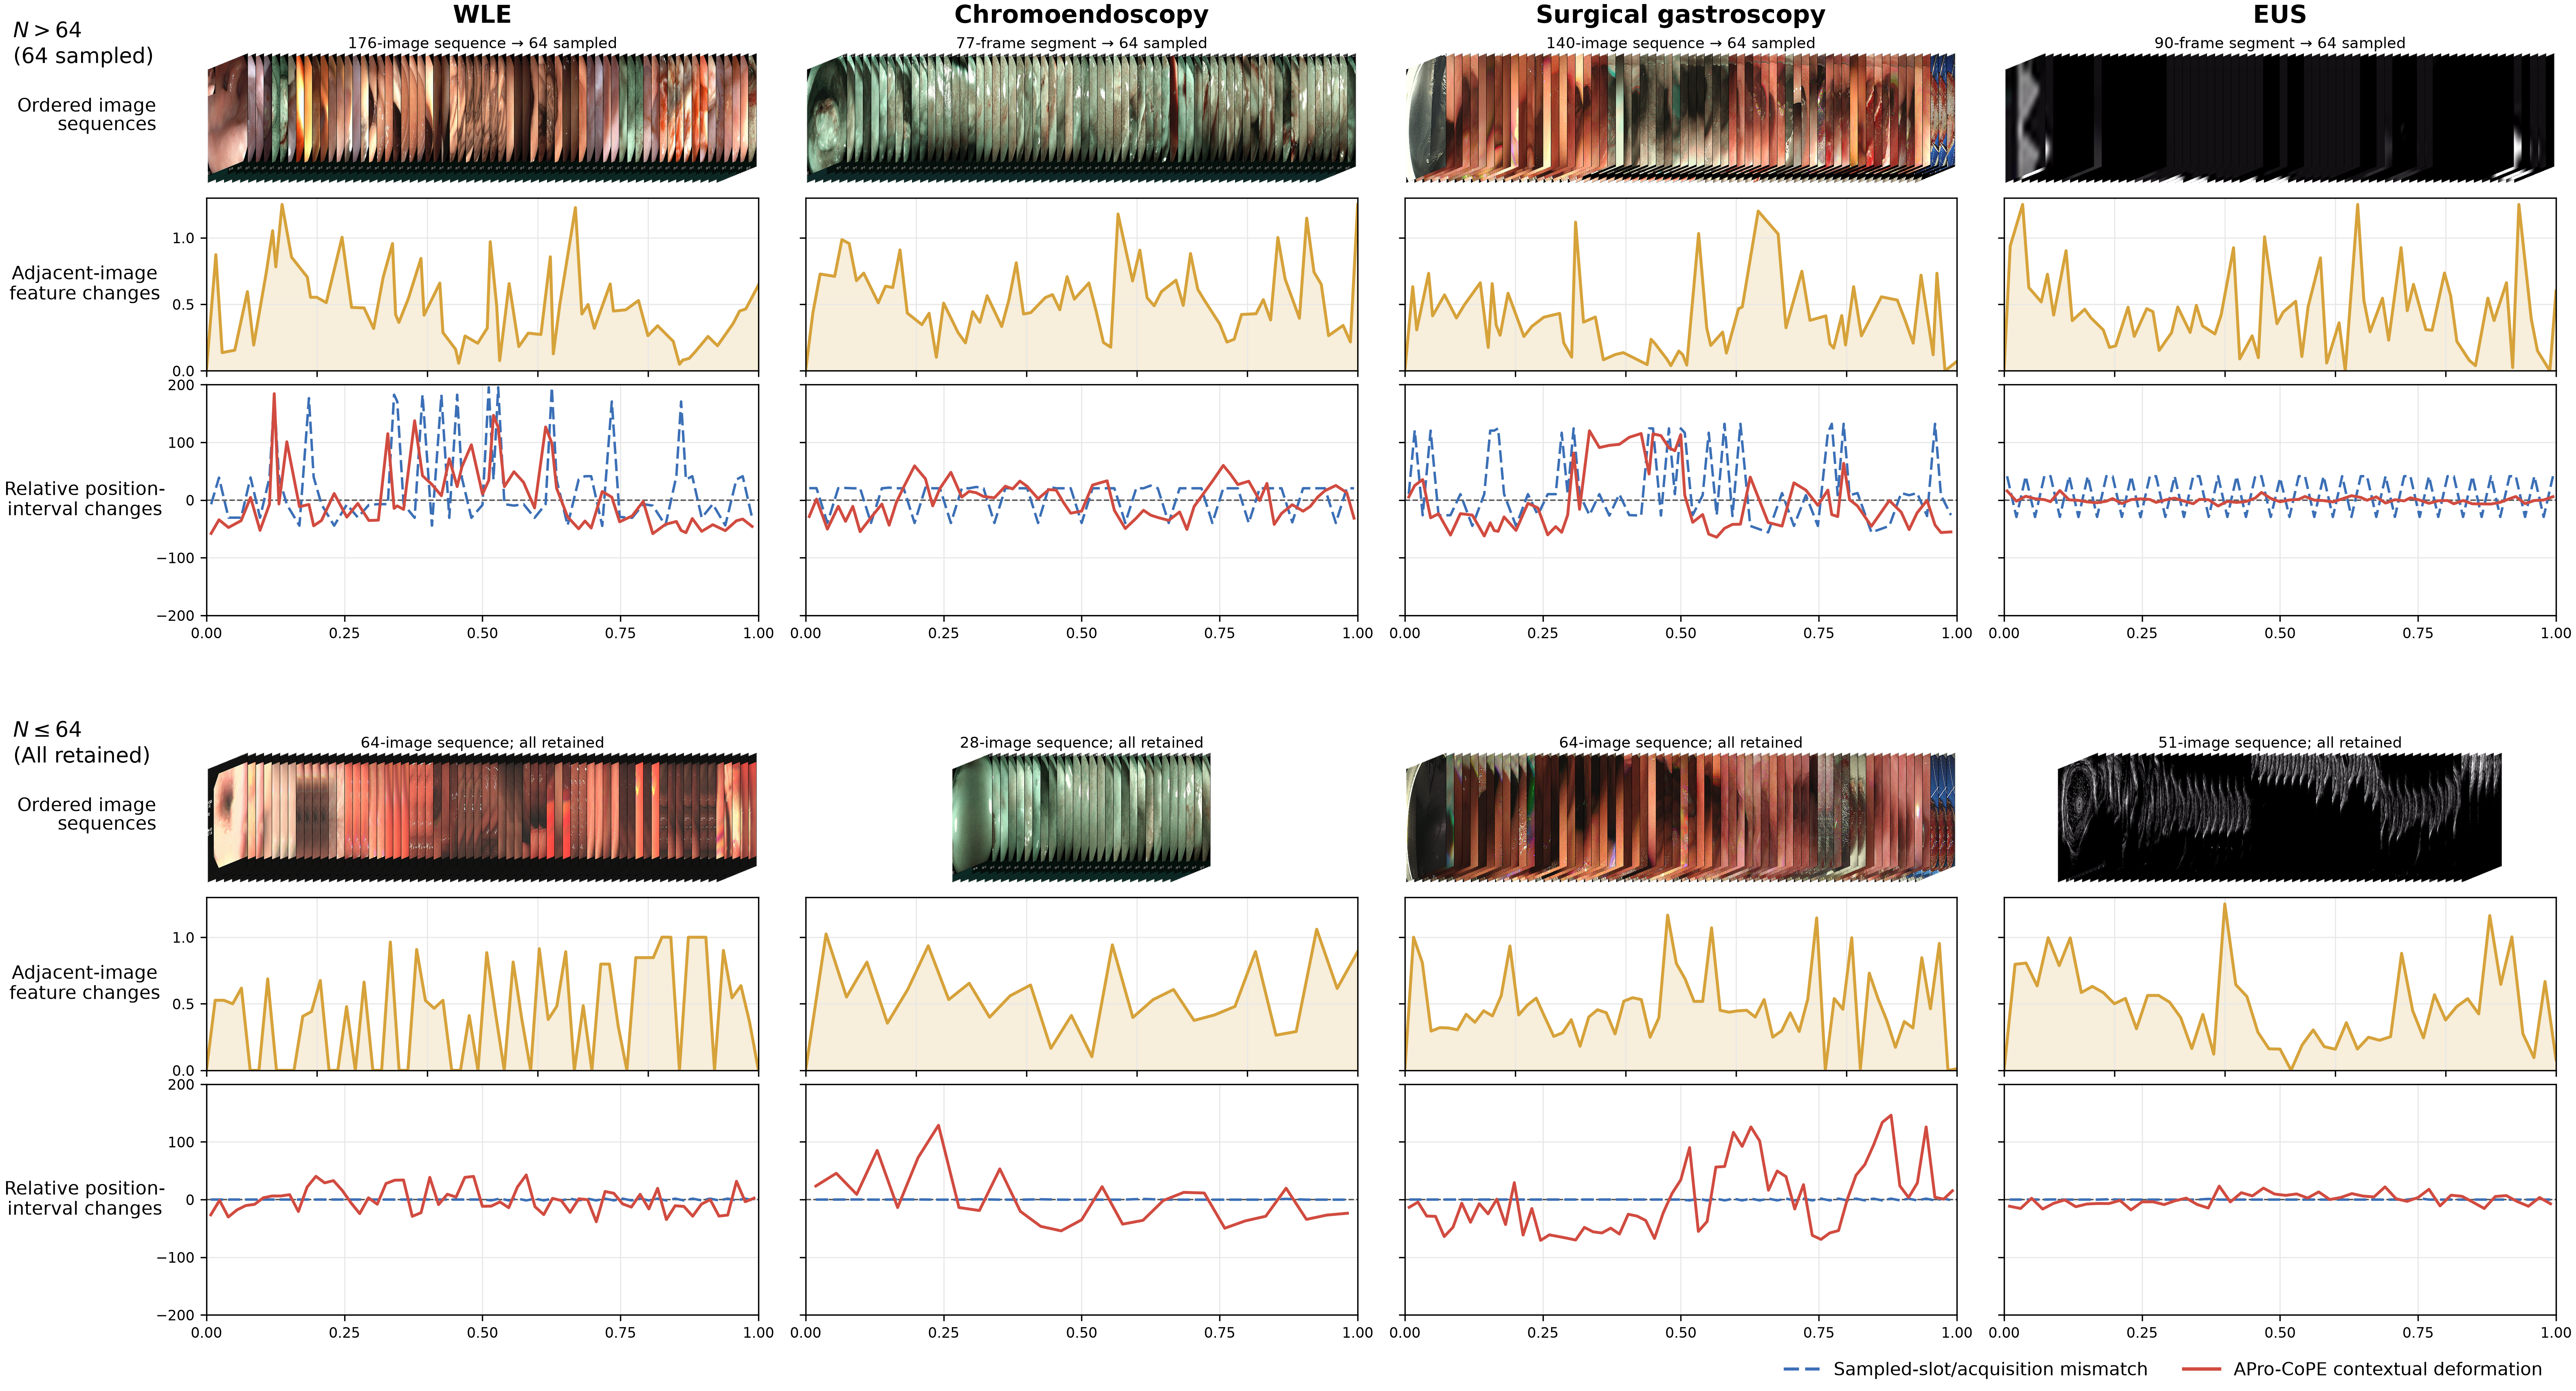
\includegraphics[width=\textwidth]{figs/apro_cope_mechanism_length_groups_four_datasets.png}
\caption{子采样与完整序列保留条件下的APro-CoPE定性可视化。最大图像预算为$T=64$时，上组在$N>64$时均匀采样64张图像，下组在$N\leq64$时保留完整序列。\label{fig:apro_cope_length_groups}}
\end{figure*}

为定性展示APro-CoPE如何针对均匀子采样序列和完整保留序列构建采集锚定、内容自适应的位置关系，本文在最大图像预算$T=64$下选取代表性检查进行可视化。图像数量超过64张的检查采用64张图像的均匀子采样表示，同时保留入选图像的原始采集顺序和采集索引；图像数量至多为64张的检查保留完整图像序列。图~\ref{fig:apro_cope_length_groups}通过四个胃镜数据集的示例展示这两种输入构建方式。对于每个示例，图像条带为实际输入模型的有序序列，橙色曲线表示相邻图像之间的特征变化，蓝色虚线表示从原始采集位置到均匀采样槽位的相对间隔变化，红色实线表示从采集锚点到APro-CoPE上下文坐标的相对间隔变化。因此，蓝色曲线刻画输入构建过程中产生的位置变化，红色曲线刻画模型随后进行的内容自适应调整。

均匀子采样保留了入选图像在完整采集序列中的位置，因此蓝色曲线呈现明显波动；完整序列保留使图像顺序与采样槽位直接对应，蓝色曲线相应接近于零。在这些采集锚点基础上，两种输入构建方式下的红色曲线均形成了面向具体检查的变化模式，展示APro-CoPE如何根据图像内容重新分配上下文位置间隔。红色变形模式与相邻图像之间视觉变化的连续性相对应，反映由持续图像转变驱动的内容自适应间隔调整。特别是在EUS示例中，若干孤立的相邻图像特征变化峰值与较小的整体红色调整同时出现；相比之下，WLE、染色胃镜和手术胃镜示例在包含持续视觉变化的序列区段呈现更明显的调整。上述结果体现APro-CoPE对均匀子采样输入和完整序列输入的检查特异性位置建模。

\subsubsection{APro-CoPE对检查级预测质量的影响}

图~\ref{fig:apro_cope_prediction_distributions}比较了64张图像设置下采样槽位位置编码与完整APro-CoPE在标签级准确率、真实类别置信度和Brier分数上的检查级分布。标签级准确率表示三个二元标签中预测正确的比例；真实类别置信度表示模型赋予正确二元结果的平均概率；Brier分数表示预测概率与真实标签之间的均方误差。因此，更高的标签级准确率说明正确判定的标签更多，更高的真实类别置信度说明模型对正确结果的置信度更高，更低的Brier分数说明预测概率误差更小，三者共同反映更好的检查级预测质量。

与采样槽位位置编码相比，APro-CoPE在WLE、染色胃镜和EUS上取得了更高的平均标签级准确率，仅手术胃镜由0.9179小幅下降至0.9160。WLE、染色胃镜和手术胃镜的平均真实类别置信度同样更高，仅EUS由0.9079小幅下降至0.9025。APro-CoPE在四个数据集上的平均Brier分数均更低，其中染色胃镜的降幅最大，由0.0809降至0.0730；EUS次之，由0.0463降至0.0403。因此，APro-CoPE在多数数据集上提高了标签判定正确性和对正确结果的置信度，并在全部四个数据集上减小了预测概率误差，表明其整体改善了检查级预测质量。这些分布层面的改善也有助于解释前述实验中APro-CoPE相较于采样槽位位置编码在染色胃镜数据集上表现出的更明显优势。

\begin{figure*}[t]
\centering
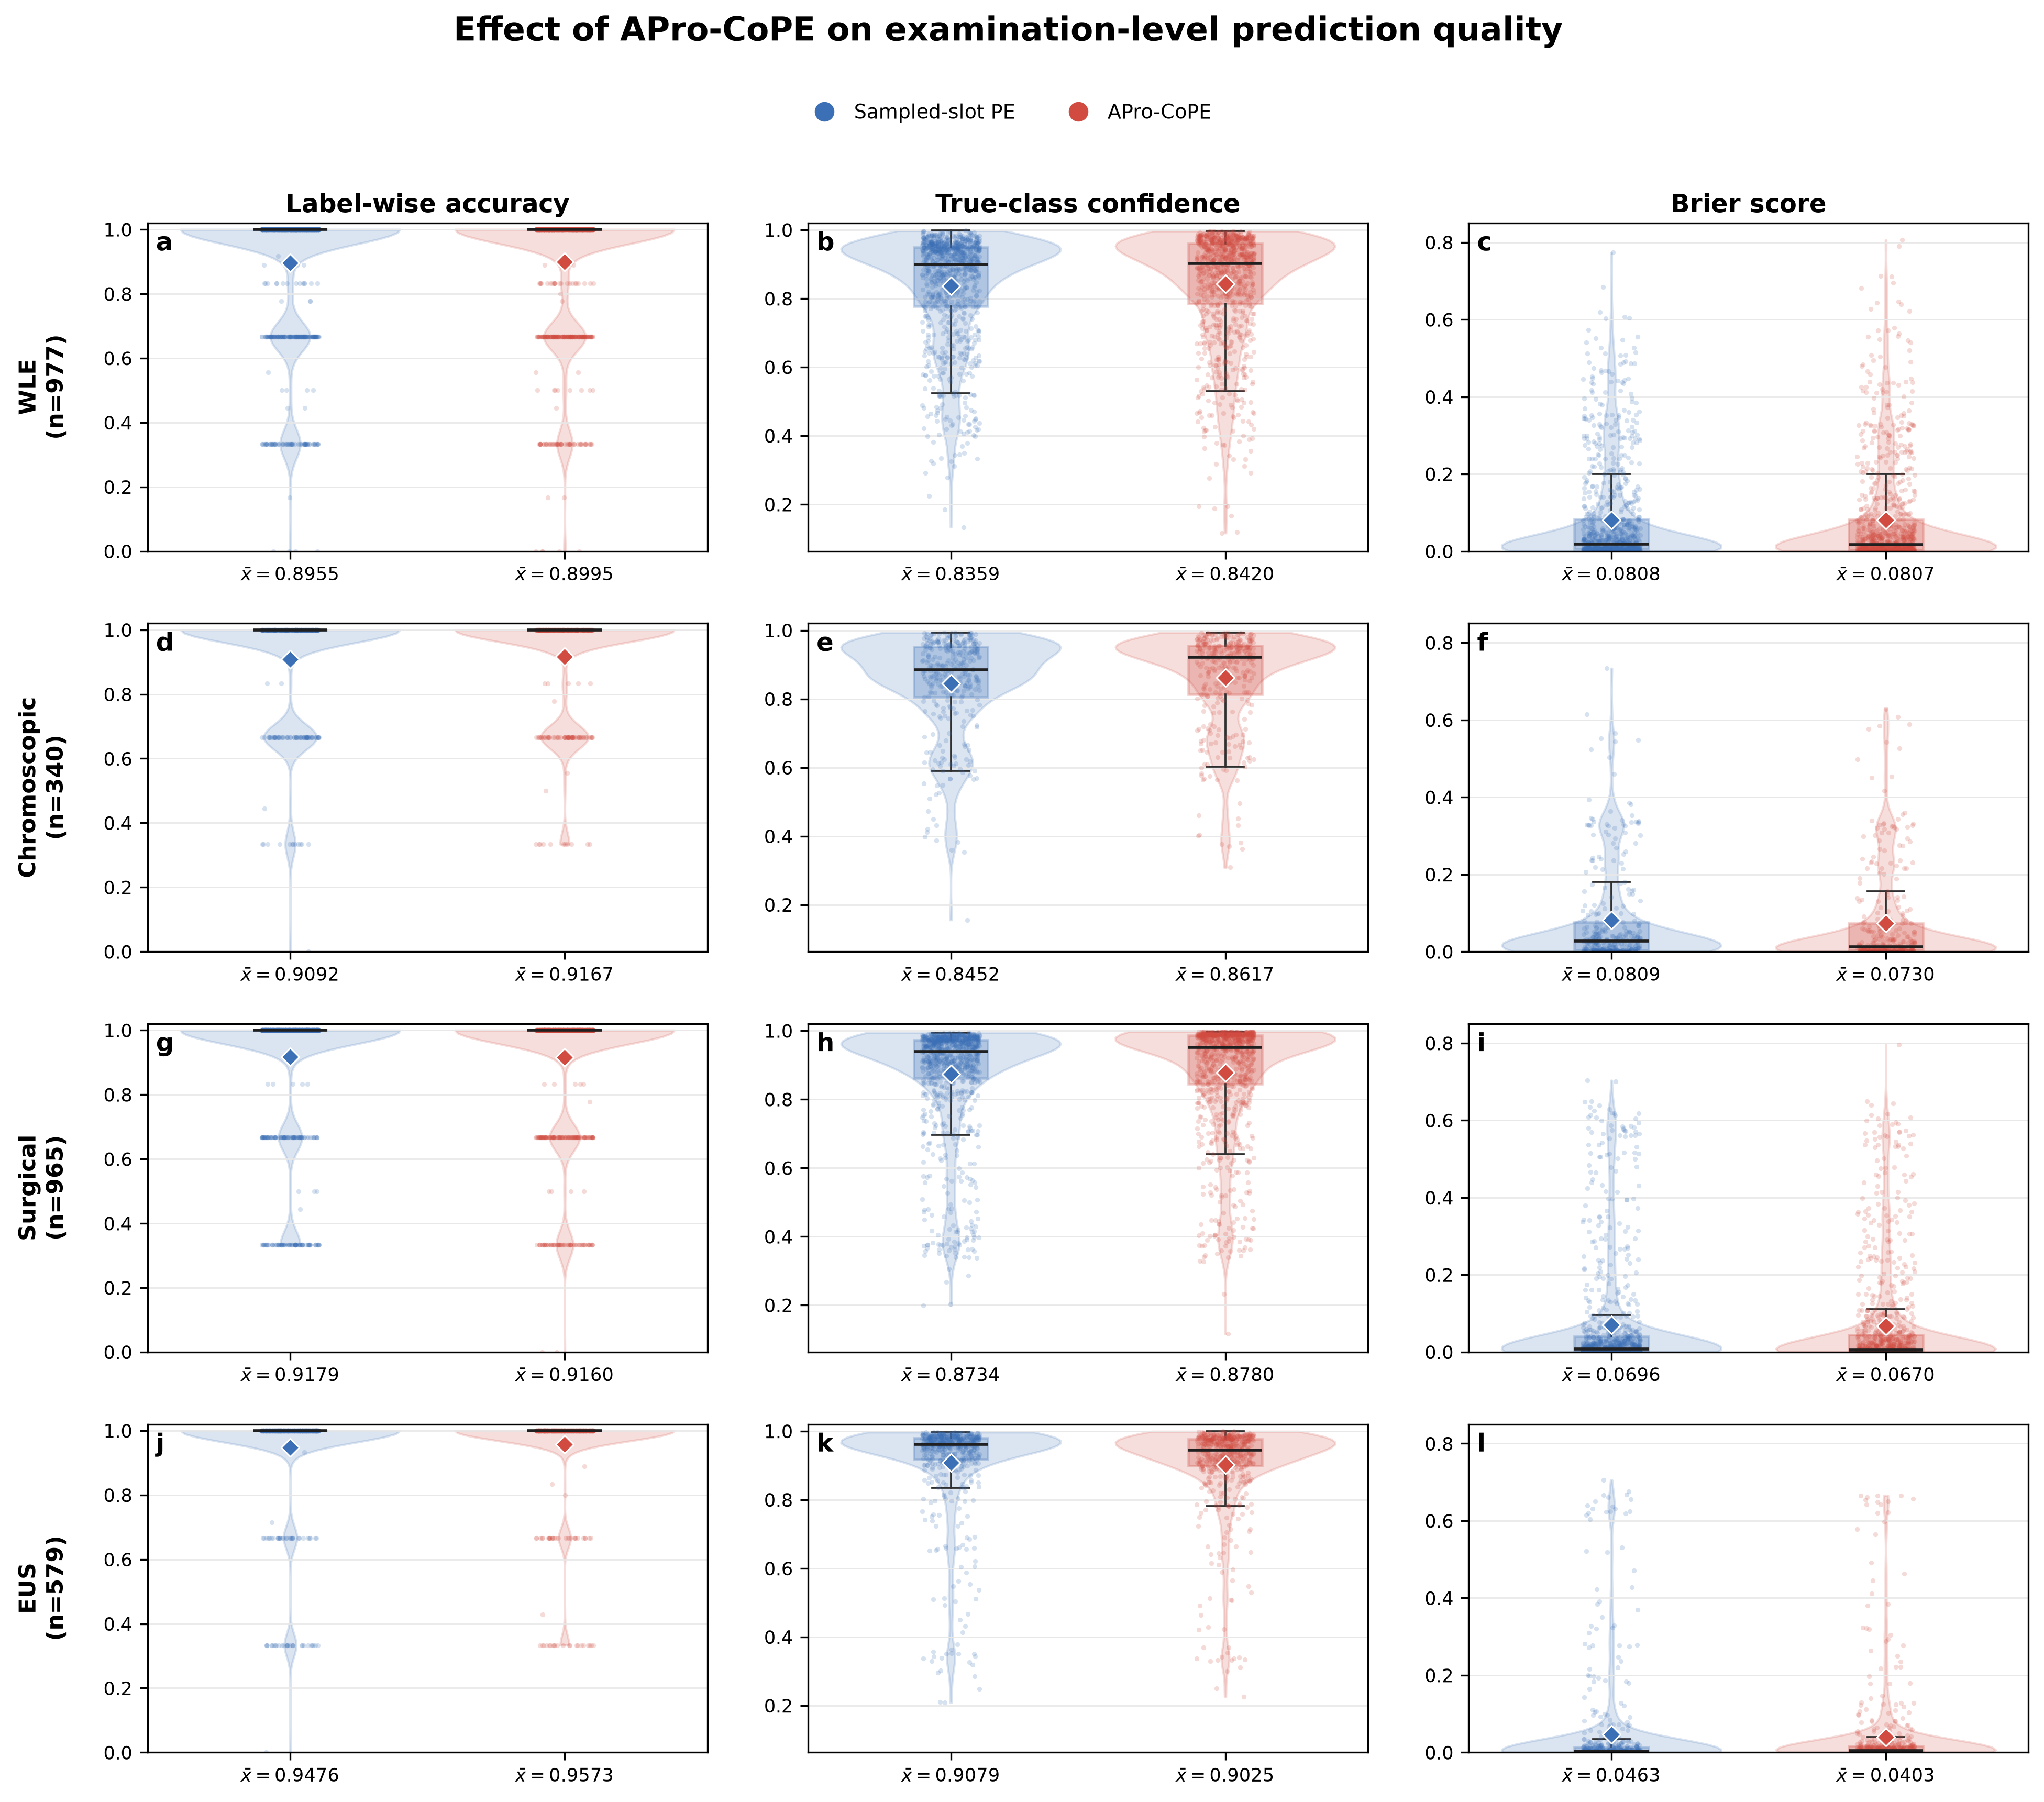
\includegraphics[width=\textwidth]{figs/apro_cope_examination_level_prediction_distributions.png}
\caption{四个胃镜数据集上APro-CoPE相对于采样槽位位置编码对检查级预测质量的影响。各行依次对应WLE、染色胃镜、手术胃镜和EUS，各列展示标签级准确率、真实类别置信度和Brier分数。每个点表示在对应留出测试折上评价的一次检查。图像数量超过64张时，在覆盖原始序列的采集顺序分层样本上对指标取平均，采样轮次最多为5次。小提琴形状表示分布，箱线表示四分位距与中位数，菱形表示算术均值，$\bar{x}$给出相应均值。标签级准确率和真实类别置信度越高越好，Brier分数越低越好。\label{fig:apro_cope_prediction_distributions}}
\end{figure*}

\subsubsection{多标签注意力MIL与标签超图推理消融}

为区分标签特异性图像聚合与高阶标签推理各自的贡献，本文开展了表~\ref{T_label_reasoning}所示的针对性消融实验。实验以不进行标签推理的共享注意力MIL为起点，引入多标签注意力MIL，并进一步比较不使用标签推理、使用普通可学习标签图以及使用本文标签超图的配置。

将共享注意力MIL替换为多标签注意力MIL后，四个数据集上的宏平均F1均得到提升，增幅为0.56--0.61个百分点。进一步加入普通标签图带来0.56--0.62个百分点的增益，而将普通标签图替换为标签超图后又取得1.86--3.59个百分点的更大提升。采用多标签注意力与标签超图推理组合的模型配置在所有数据集上均取得最高宏平均F1，相较共享注意力基线提高3.09--4.76个百分点，支持标签特异性图像聚合与高阶标签推理具有互补作用。

\begin{table*}[t]
\scriptsize\tabletimes\centering
\caption{四个胃镜数据集上多标签注意力MIL与标签超图推理的针对性消融，每次检查采样64张图像。各配置均保留采集感知视觉上下文建模、标签查询交叉注意力和门控残差融合。数值为患者分组五折宏平均F1的均值$\pm$标准差。\label{T_label_reasoning}}
\resizebox{\textwidth}{!}{%
\begin{tabular}{ll*{4}{c}}
\hline
MIL聚合 & 标签推理器 & WLE & 染色胃镜 & 手术胃镜 & EUS \\
\hline
Shared attention & -- & \tresult{0.8840}{0.0148} & \tresult{0.8401}{0.0465} & \tresult{0.8054}{0.0479} & \tresult{0.8732}{0.0691} \\
Multi-label attention & -- & \tresult{0.8901}{0.0141} & \tresult{0.8460}{0.0438} & \tresult{0.8110}{0.0447} & \tresult{0.8792}{0.0658} \\
Multi-label attention & Label graph & \tresult{0.8963}{0.0135} & \tresult{0.8518}{0.0406} & \tresult{0.8166}{0.0408} & \tresult{0.8853}{0.0623} \\
Multi-label attention & Label hypergraph & \tresult{\textbf{0.9149}}{\textbf{0.0114}} & \tresult{\textbf{0.8877}}{\textbf{0.0168}} & \tresult{\textbf{0.8456}}{\textbf{0.0224}} & \tresult{\textbf{0.9064}}{\textbf{0.0474}} \\
\hline
\end{tabular}
}
\par\raggedright\scriptsize MIL, multiple instance learning; Label graph denotes an ordinary learnable label graph.
\end{table*}

为判断表~\ref{T_label_reasoning}中的性能增益是否伴随标签特异性的视觉证据分配，本文比较了四个胃镜数据集中不同标签图像证据集合的重叠情况（图~\ref{fig:label_evidence_overlap}）。我们模型的多标签注意力模块在各检查场景下均保持在证据分离能力最强的方法之列，表明该模块能够为不同疾病分配差异化的支持图像。该结果为进一步验证这些差异化证据是否选择性地参与对应标签决策提供了基础。

\begin{figure*}[t]
\centering
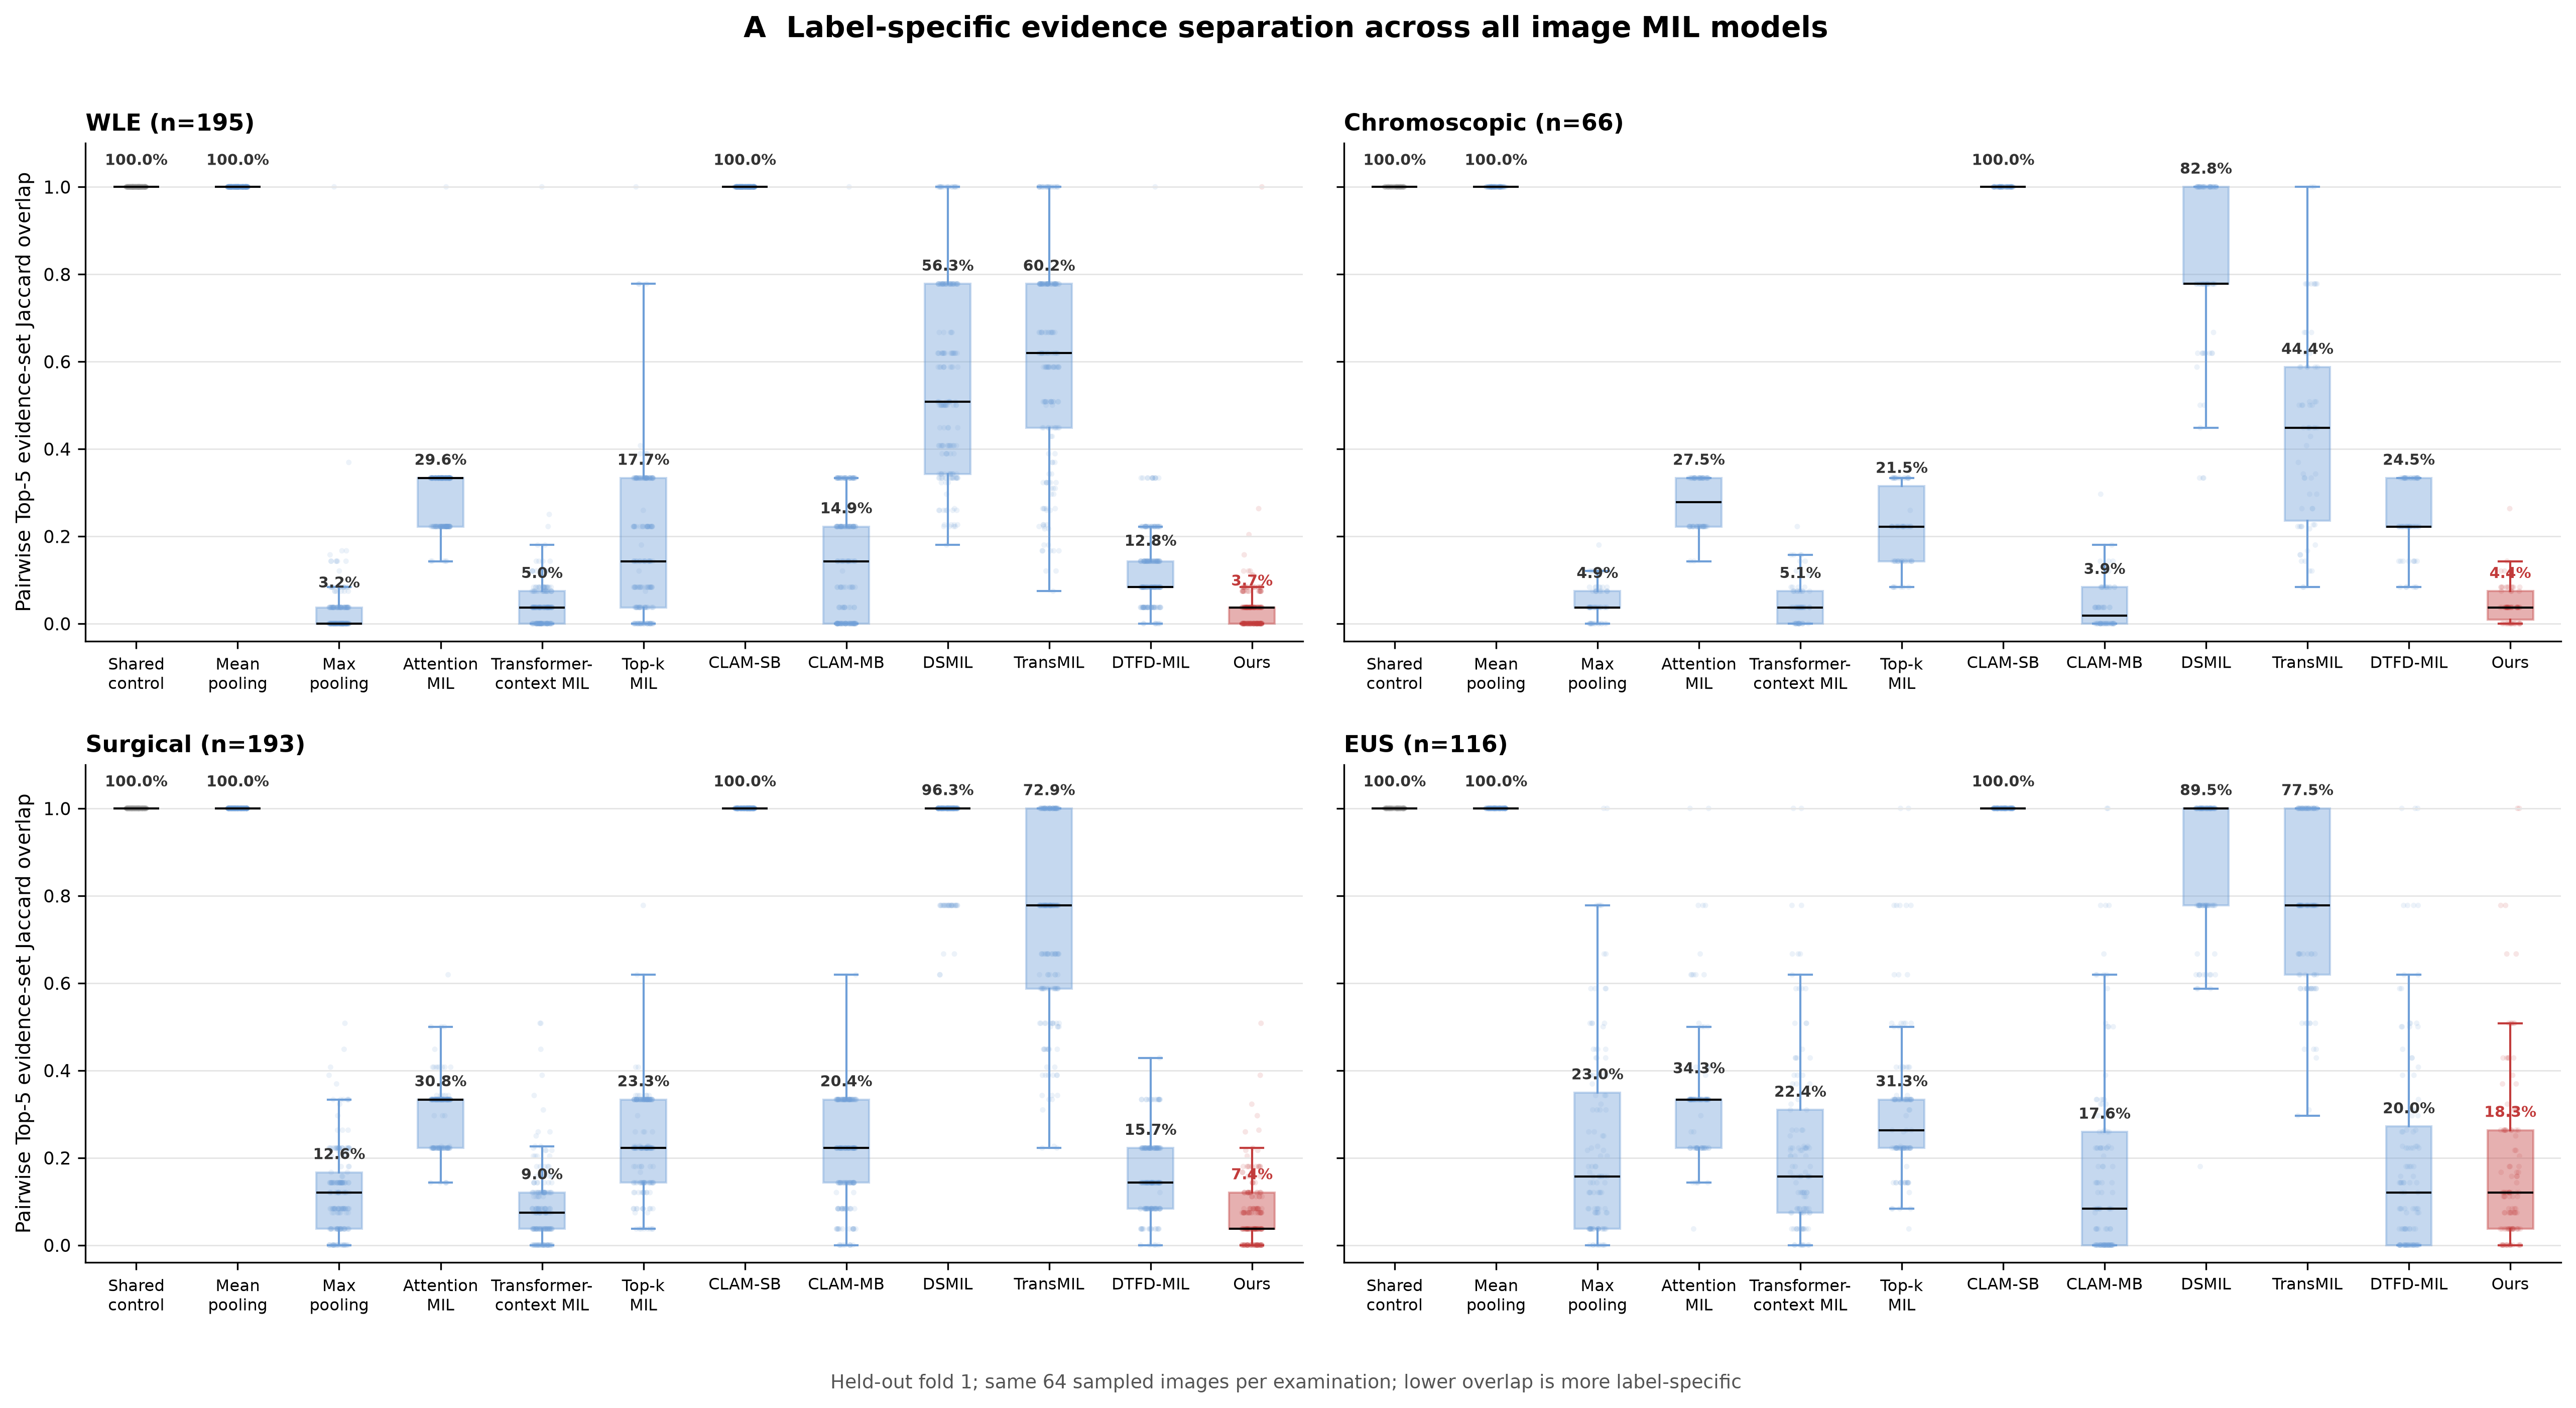
\includegraphics[width=\textwidth]{figs/label_specific_evidence_overlap_four_datasets.png}
\caption{不同MIL架构的标签特异性图像证据分离情况。对折1留出测试集中的每次检查，使用同一组最多64张均匀采样图像，分别按照三个标签进行排序，并计算三组Top-5证据集合之间的平均两两Jaccard重叠率。每个点表示一次检查，箱线表示四分位距与中位数，百分比表示算术均值。重叠率越低表示标签特异性支持证据的分离越强。\label{fig:label_evidence_overlap}}
\end{figure*}

为进一步评估分离后的证据是否选择性地参与对应标签决策，本文开展了标签定向删除实验（图~\ref{fig:label_targeted_deletion}）。与共享注意力对照相比，我们模型的多标签注意力模块在大多数检查场景中呈现出更强的对角线集中趋势。当删除某一标签对应的高注意力证据后，模型的决策影响更多集中于该标签自身，说明该模块能够学习具有标签特异性的视觉证据。综合较低的标签间证据重叠与更强的标签特异性决策影响，结果表明标签证据分离和标签特异性决策能够减少不同标签之间的证据干扰，从而促进采用多标签注意力与标签超图推理组合的模型配置获得更高的宏平均F1。

\begin{figure*}[t]
\centering
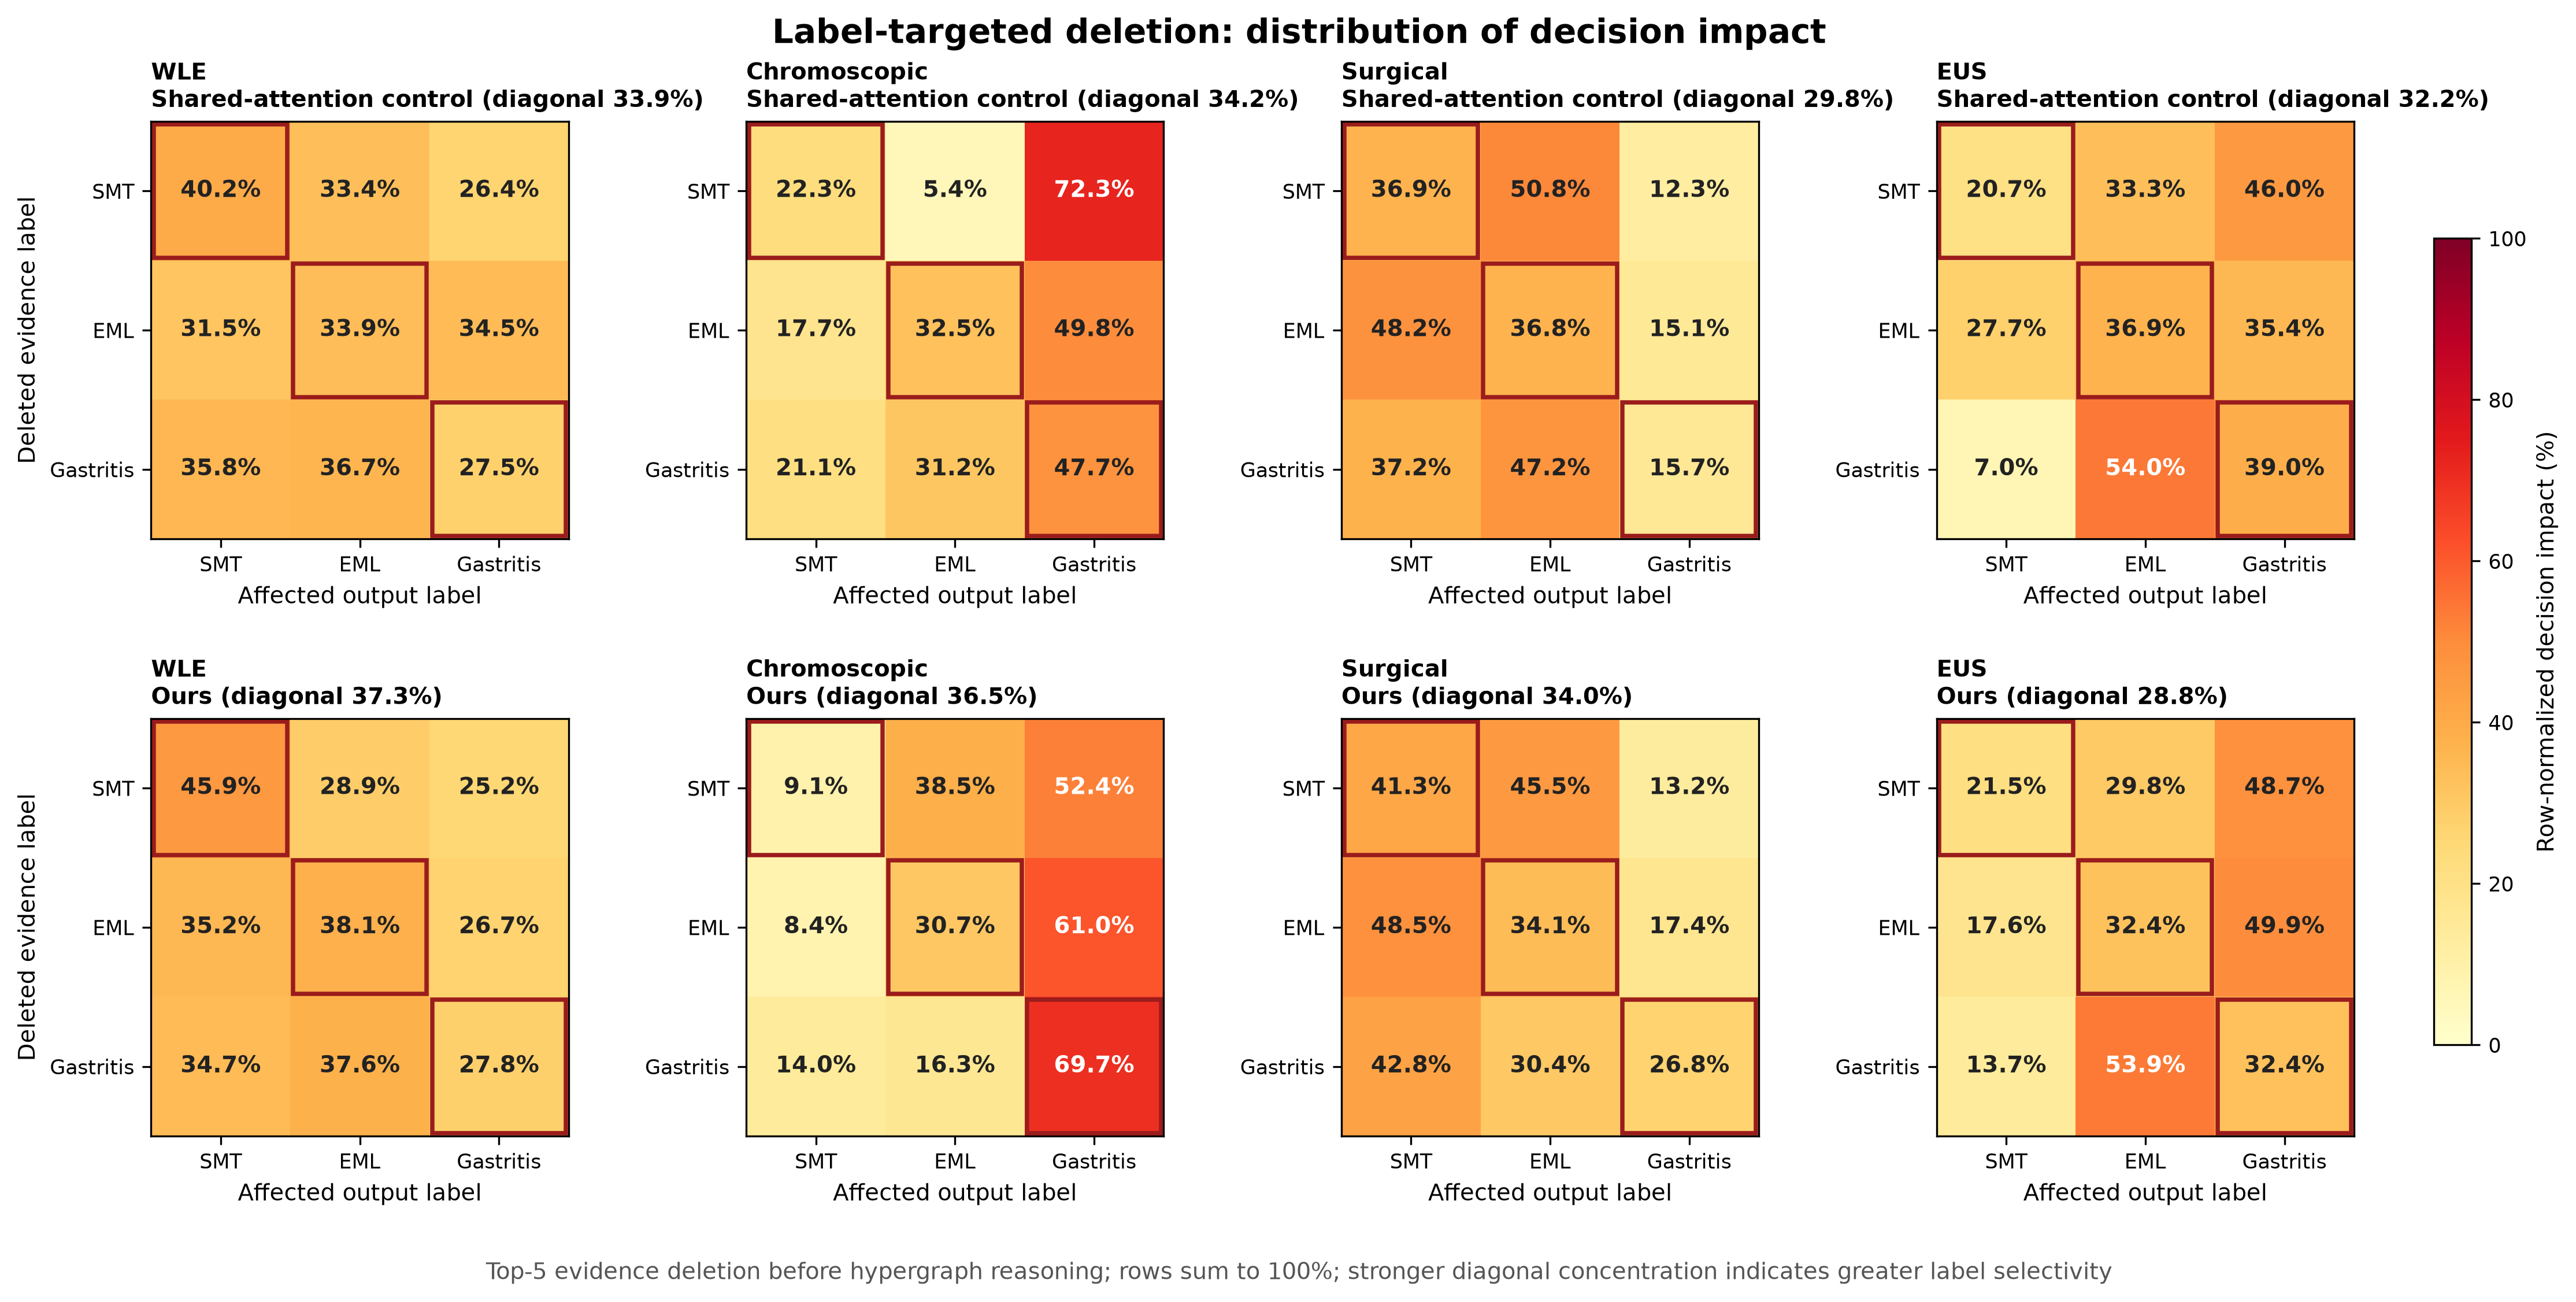
\includegraphics[width=\textwidth]{figs/label_targeted_deletion_selectivity_four_datasets.png}
\caption{四个胃镜数据集上的标签定向删除分析。对每个被删除证据的标签（行），在标签超图推理前移除其Top-5注意力图像，并将由此产生的决策影响分配至三个输出标签（列），随后在每行内归一化为100\%。上排为共享注意力对照，下排为所提出模型。红色边框标记被删除标签与受影响标签一致的位置；对角线越集中表示标签特异性决策选择性越强。\label{fig:label_targeted_deletion}}
\end{figure*}

为更直接考察标签超图推理在共存发现检查中的作用，本文进一步按照每次检查仅包含一个阳性目标或包含多个共阳性目标，对阳性标签置信度进行分层比较（图~\ref{fig:label_hypergraph_copositive_confidence}）。单阳性组作为参照。在该组中，标签超图在部分数据集上的置信度略低于普通标签图，这与其主要面向共存疾病高阶关系、而非孤立阳性标签进行设计的定位一致。相比之下，在共阳性组中，标签超图推理在四个数据集上均取得最高的平均阳性标签置信度，并一致高于无标签推理和普通标签图。该结果表明，高阶标签交互能够增强模型对共存疾病证据的整合，从而促进表~\ref{T_label_reasoning}中多标签注意力与标签超图推理组合获得更高的宏平均F1。

\begin{figure*}[t]
\centering
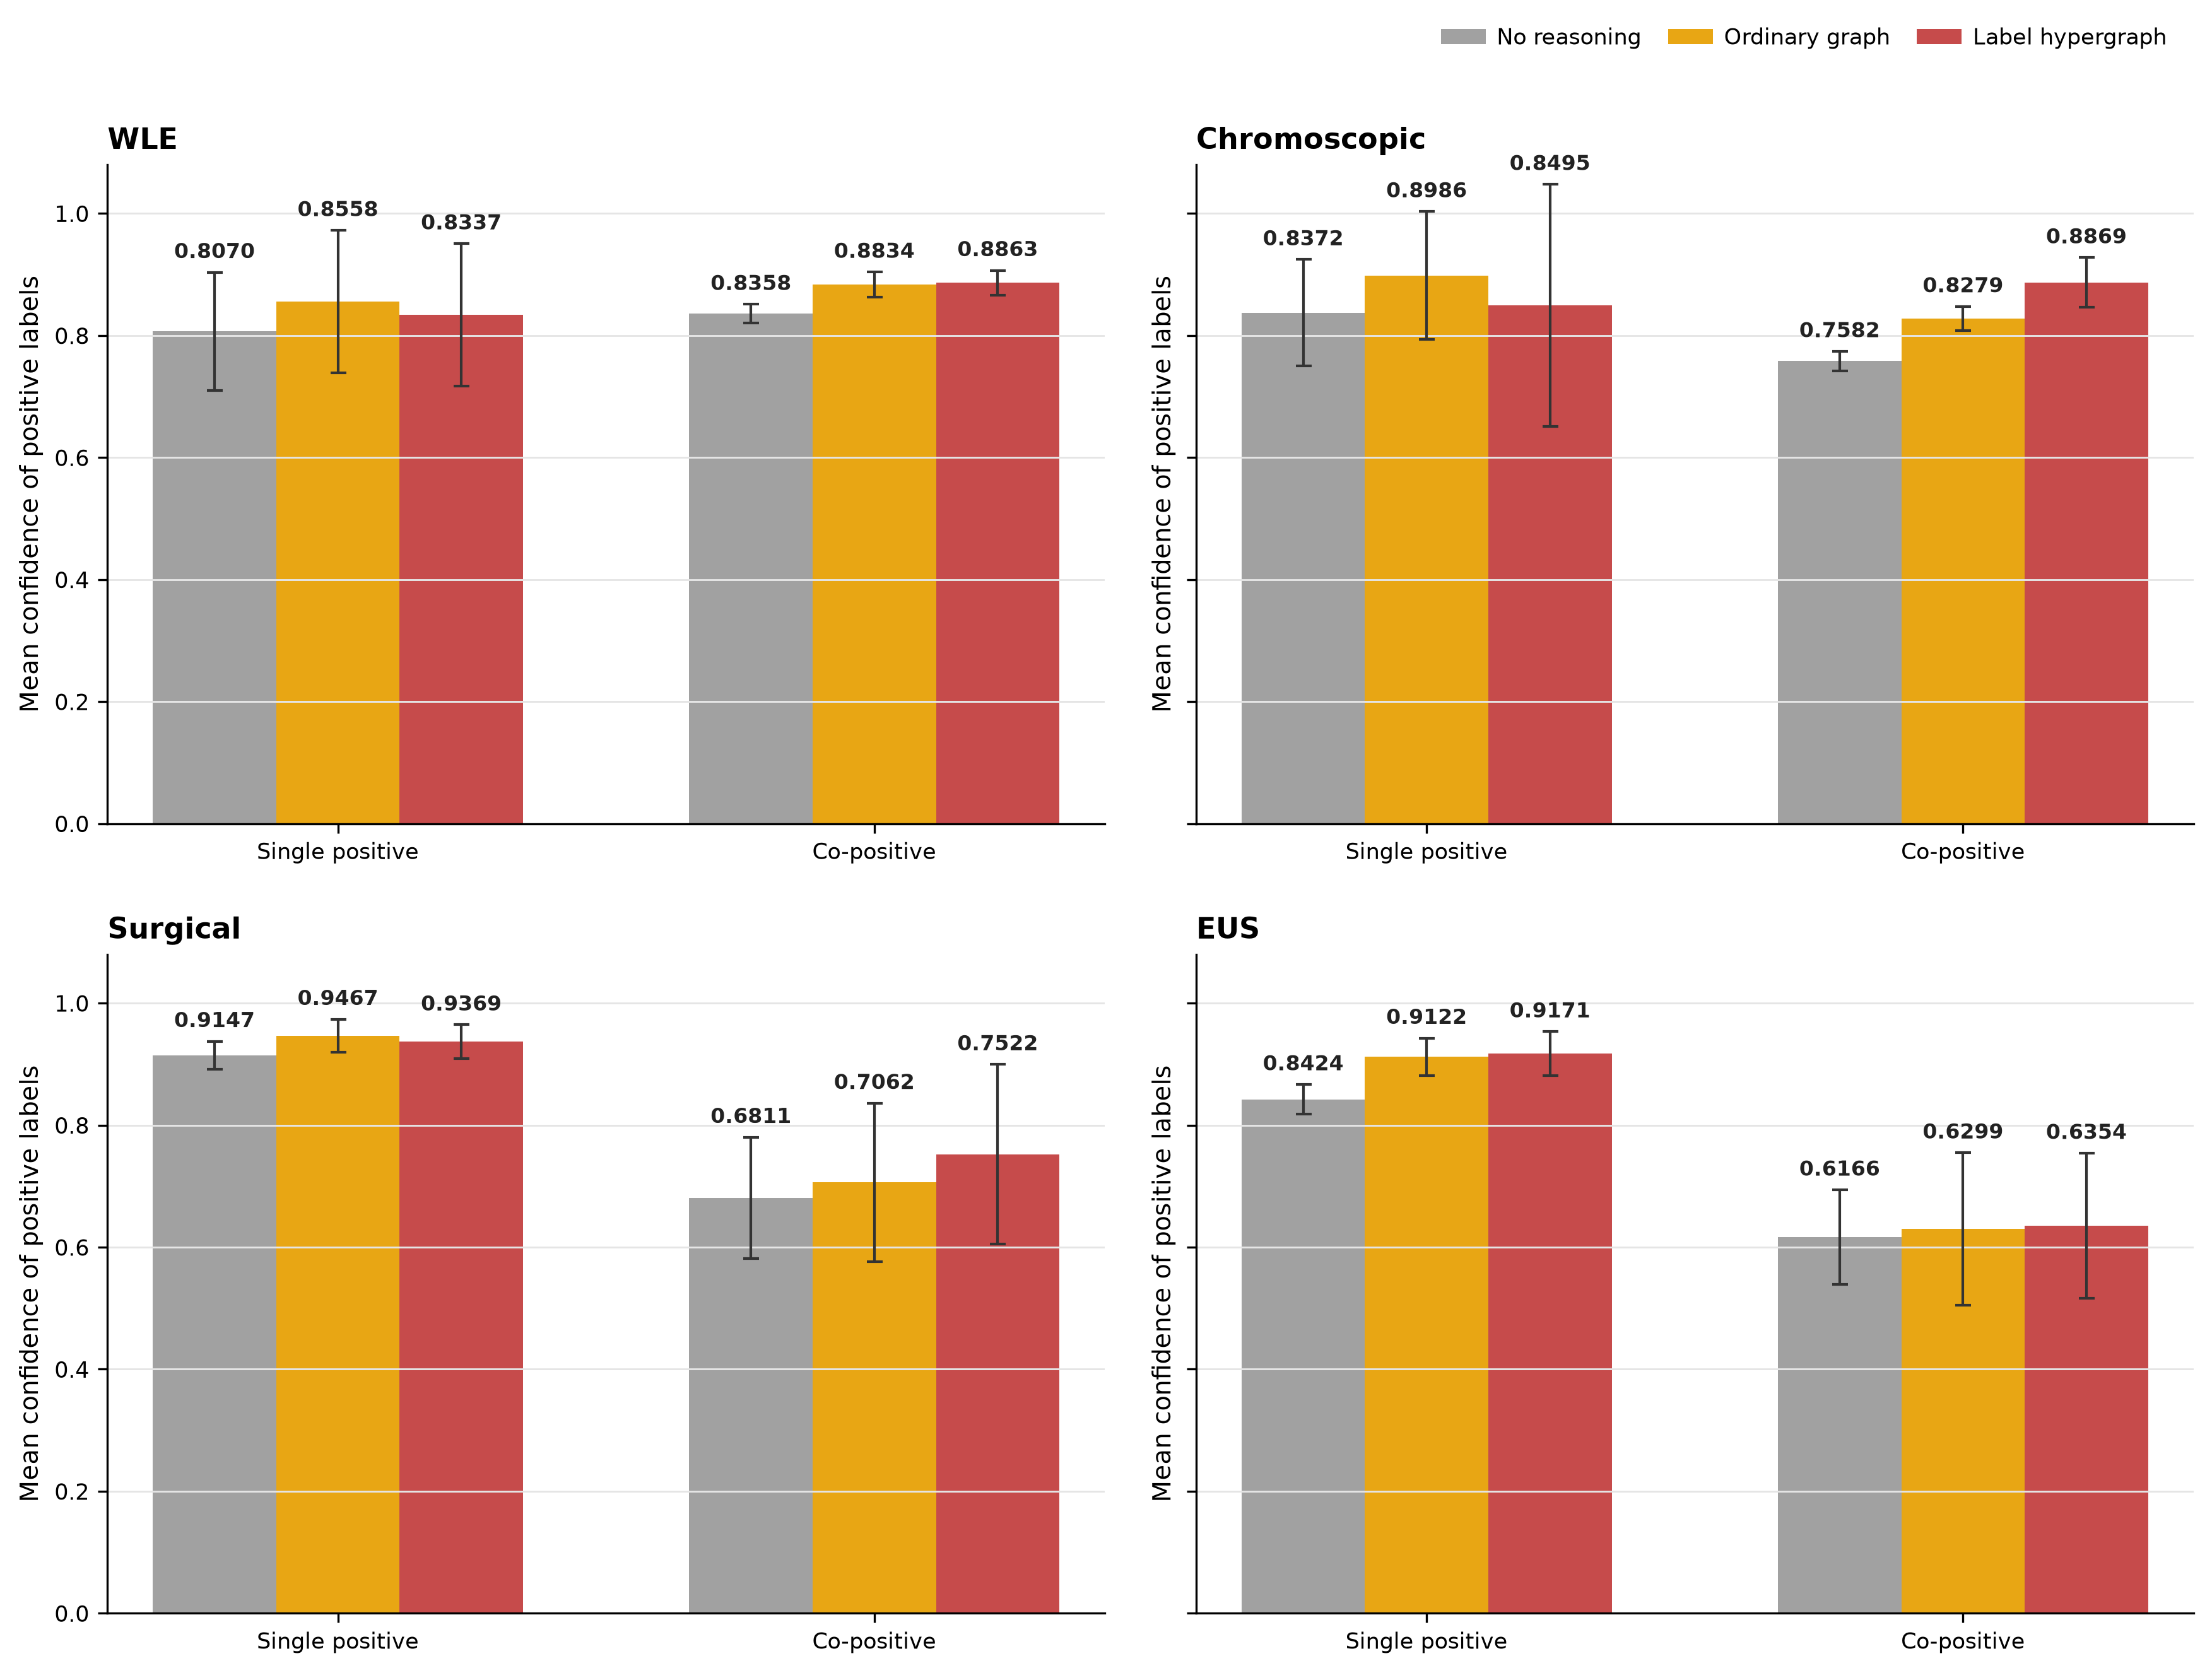
\includegraphics[width=\textwidth]{figs/label_hypergraph_copositive_confidence_four_datasets.png}
\caption{四个胃镜数据集上不同标签集合复杂度下的阳性标签置信度。依据阳性目标标签数量将检查分为单阳性组和共阳性组。柱形表示模型赋予阳性标签的平均置信度，误差线表示95\%置信区间。比较配置均采用多标签注意力，仅标签推理机制不同。\label{fig:label_hypergraph_copositive_confidence}}
\end{figure*}

\subsubsection{标签条件跨模态检索与自适应残差融合消融}

为区分标签条件文本检索与自适应残差融合各自及联合产生的贡献，本文针对标签查询交叉注意力（LQCA）和门控残差融合（GRF）开展$2\times2$消融实验。实验以两个组件均未启用的配置为基线，分别考察仅启用LQCA、仅启用GRF以及同时启用二者的配置。实验结果汇总于表~\ref{T_crossmodal_fusion}。

标签查询检索和门控融合均优于视觉路径，二者联合时在所有数据集上取得最高宏平均F1，提升幅度为2.42--4.40个百分点。上述结果支持标签条件检索与对所检索文本证据进行自适应控制具有互补作用。

\begin{table*}[t]
\scriptsize\tabletimes\centering
\caption{四个胃镜数据集上标签查询交叉注意力与门控残差融合的$2\times2$消融，每次检查采样64张图像。各配置均保留基于APro-CoPE的采集感知上下文建模和标签超图推理。数值为患者分组五折宏平均F1的均值$\pm$标准差。\label{T_crossmodal_fusion}}
\resizebox{\textwidth}{!}{%
\begin{tabular}{cc*{4}{c}}
\hline
文本检索 & 残差融合 & WLE & 染色胃镜 & 手术胃镜 & EUS \\
\hline
-- & -- & \tresult{0.8907}{0.0110} & \tresult{0.8437}{0.0524} & \tresult{0.8055}{0.0600} & \tresult{0.8769}{0.0675} \\
LQCA & -- & \tresult{0.9031}{0.0128} & \tresult{0.8658}{0.0320} & \tresult{0.8267}{0.0456} & \tresult{0.8921}{0.0567} \\
-- & GRF & \tresult{0.9056}{0.0119} & \tresult{0.8693}{0.0437} & \tresult{0.8299}{0.0491} & \tresult{0.8940}{0.0538} \\
LQCA & GRF & \tresult{\textbf{0.9149}}{\textbf{0.0114}} & \tresult{\textbf{0.8877}}{\textbf{0.0168}} & \tresult{\textbf{0.8456}}{\textbf{0.0224}} & \tresult{\textbf{0.9064}}{\textbf{0.0474}} \\
\hline
\end{tabular}
}
\par\raggedright\scriptsize LQCA, label-query cross-attention; GRF, gated residual fusion.
\end{table*}

为进一步判断LQCA带来的性能提升是否源于标签特异性的文本检索，本文比较了四个胃镜数据集中三种检索条件下的阳性标签置信度（图~\ref{fig:label_query_retrieval_specificity}）。正确条件保留对应标签查询所检索的文本表征，跨标签条件在不同标签之间互换检索表征，共享池化条件则使用统一的所见描述表征。正确标签查询对应关系下的阳性标签置信度最高，而跨标签互换或共享池化后均出现下降。该结果表明，与疾病匹配的标签查询能够检索到更有效的标签特异性文本证据，从而促进表~\ref{T_crossmodal_fusion}中采用标签查询cross-attention的模型配置获得更高的宏平均F1。

\begin{figure*}[t]
\centering
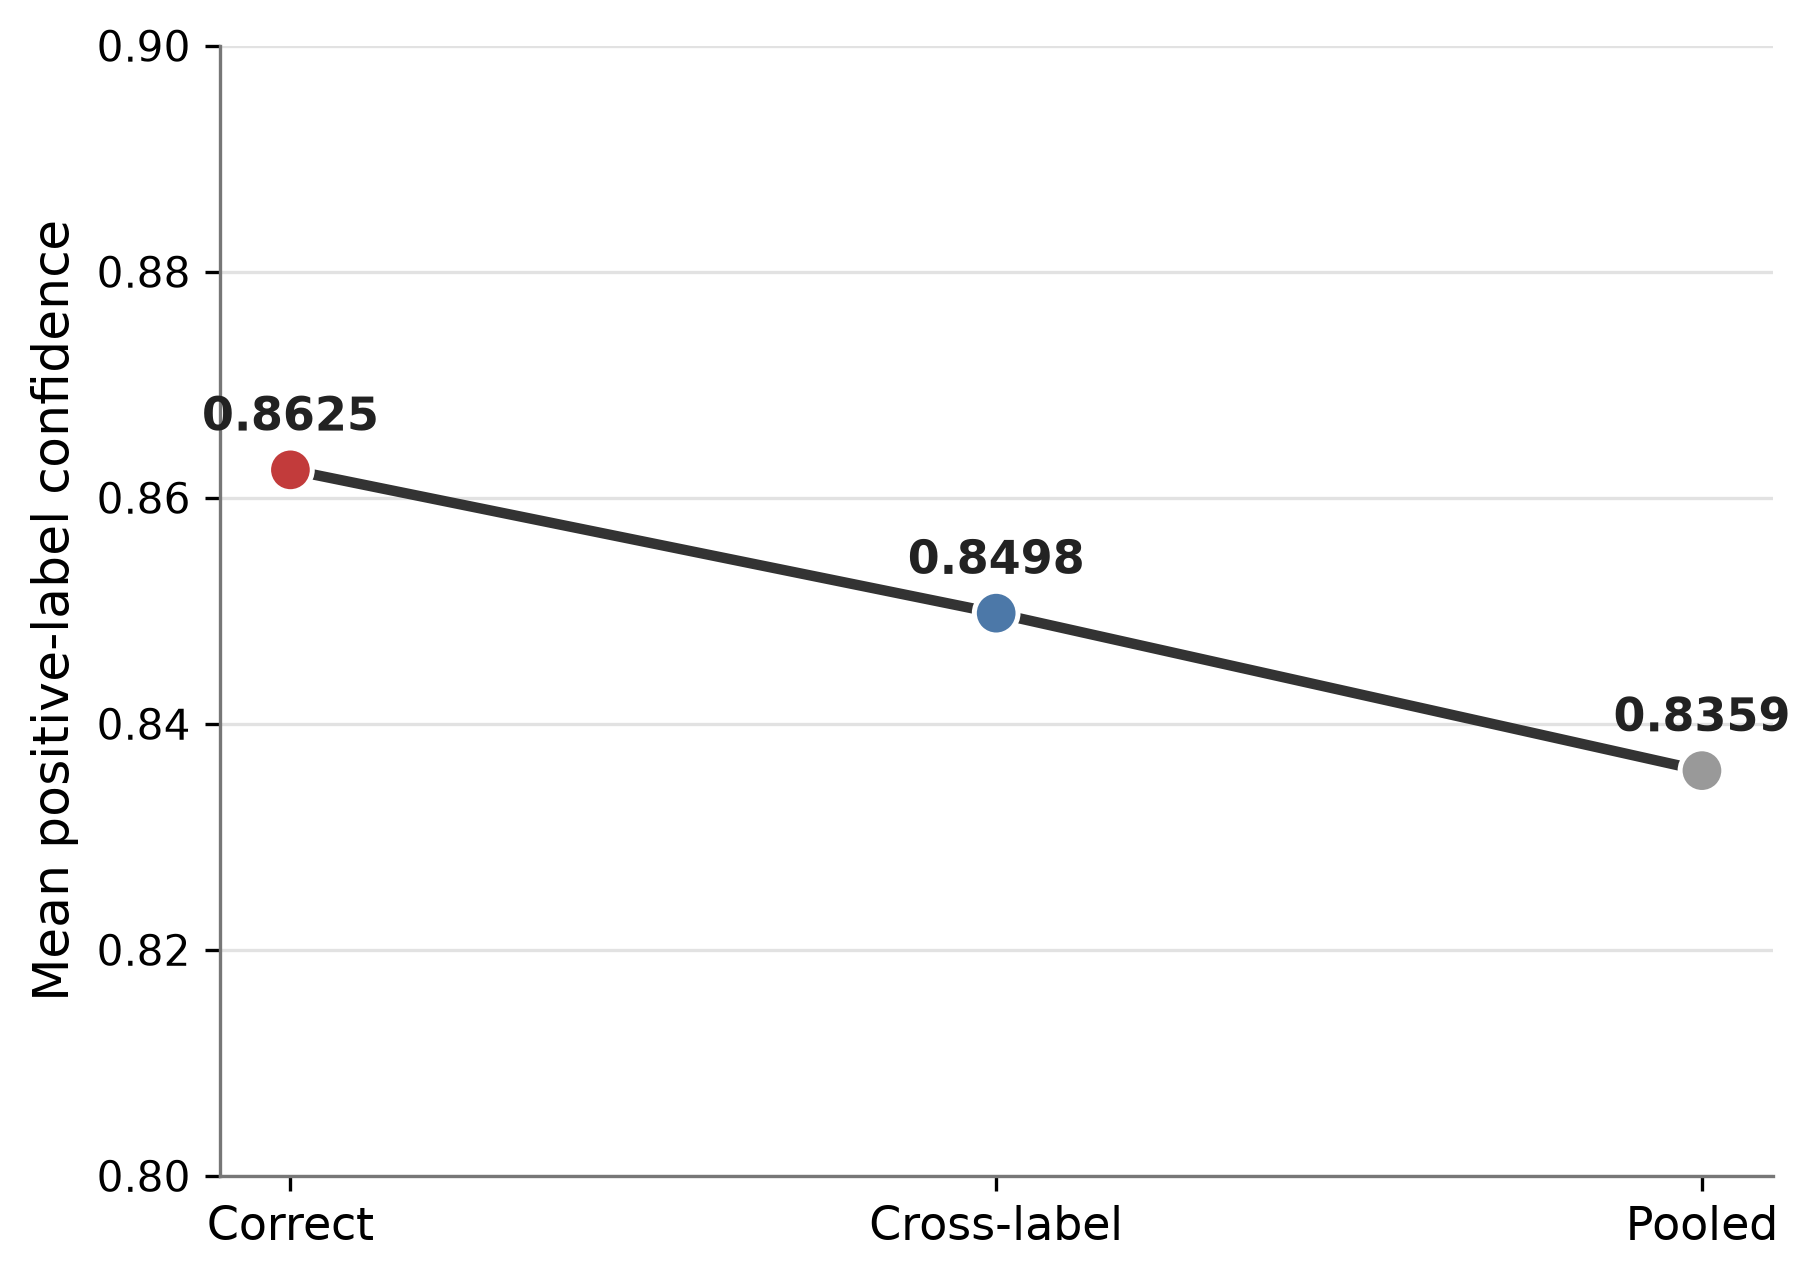
\includegraphics[width=0.62\textwidth]{figs/label_query_retrieval_specificity_four_datasets.png}
\caption{四个胃镜数据集上的标签特异性文本检索分析。正确条件保留对应标签查询所检索的文本表征，跨标签条件在不同标签之间重新分配检索表征，共享池化条件以统一所见描述表征进行替换。折线表示合并四个数据集后模型赋予阳性标签的平均置信度。\label{fig:label_query_retrieval_specificity}}
\end{figure*}

\subsubsection{主要架构组件的全因子消融}

为评价主要架构组件各自的贡献及其交互作用，本文在每次检查采样64张图像的条件下，测试基于APro-CoPE的采集感知Transformer上下文建模、标签超图推理、标签查询cross-attention和门控残差融合四个组件的全部16种组合。关闭标签超图推理时使用普通可学习标签图；同时关闭标签查询cross-attention和门控残差融合时采用视觉路径进行预测；使用cross-attention但不使用门控融合时在cross-attention后直接相加，使用门控融合但不使用cross-attention时则对池化所见描述表征进行门控融合。

在本实验中，M1表示基于APro-CoPE的采集感知Transformer上下文建模，M2表示标签超图推理，M3表示标签查询cross-attention，M4表示门控残差融合。表~\ref{T_factorial}的结果表明，相对于不使用四个组件的基线，单独启用基于APro-CoPE的采集感知Transformer上下文建模在每个数据集上带来的宏平均F1变化均小于0.3个百分点。标签超图推理带来0.70--1.37个百分点的稳定提升，而标签查询cross-attention和门控残差融合的单独增益更大，分别达到1.61--2.93和1.76--3.36个百分点。标签超图推理与门控残差融合的组合在四个数据集上均为表现最好的双组件配置。全部四个组件同时启用时，各数据集均取得最高宏平均F1，并相对于无组件基线在WLE、染色胃镜、手术胃镜和EUS上分别提高2.78、5.22、4.51和3.34个百分点。

\begin{table*}[t]
\scriptsize\tabletimes\centering
\caption{四个胃镜数据集上四个主要架构组件的全因子消融，每次检查采样64张图像。数值为患者分组五折宏平均F1的均值$\pm$标准差。M1表示基于APro-CoPE的采集感知Transformer上下文建模，M2表示标签超图推理，M3表示标签查询交叉注意力，M4表示门控残差融合。M1内部的位置设计选择见表~\ref{T3_apro}。\label{T_factorial}}
\resizebox{\textwidth}{!}{%
\begin{tabular}{*{4}{c}*{4}{c}}
\hline
M1 & M2 & M3 & M4 & WLE & Chromoscopic & Surgical & EUS \\
\hline
-- & -- & -- & -- & \tresult{0.8871}{0.0124} & \tresult{0.8355}{0.0508} & \tresult{0.8005}{0.0734} & \tresult{0.8730}{0.0715} \\
$\checkmark$ & -- & -- & -- & \tresult{0.8874}{0.0134} & \tresult{0.8383}{0.0481} & \tresult{0.8000}{0.0639} & \tresult{0.8729}{0.0839} \\
-- & $\checkmark$ & -- & -- & \tresult{0.8941}{0.0134} & \tresult{0.8492}{0.0583} & \tresult{0.8110}{0.0667} & \tresult{0.8816}{0.0581} \\
-- & -- & $\checkmark$ & -- & \tresult{0.9032}{0.0115} & \tresult{0.8648}{0.0560} & \tresult{0.8252}{0.0563} & \tresult{0.8935}{0.0633} \\
-- & -- & -- & $\checkmark$ & \tresult{0.9047}{0.0135} & \tresult{0.8691}{0.0479} & \tresult{0.8304}{0.0619} & \tresult{0.8953}{0.0711} \\
$\checkmark$ & $\checkmark$ & -- & -- & \tresult{0.8907}{0.0110} & \tresult{0.8437}{0.0524} & \tresult{0.8055}{0.0600} & \tresult{0.8769}{0.0675} \\
$\checkmark$ & -- & $\checkmark$ & -- & \tresult{0.8964}{0.0107} & \tresult{0.8539}{0.0381} & \tresult{0.8149}{0.0457} & \tresult{0.8851}{0.0668} \\
$\checkmark$ & -- & -- & $\checkmark$ & \tresult{0.8981}{0.0124} & \tresult{0.8532}{0.0448} & \tresult{0.8161}{0.0621} & \tresult{0.8874}{0.0626} \\
-- & $\checkmark$ & $\checkmark$ & -- & \tresult{0.9017}{0.0119} & \tresult{0.8640}{0.0385} & \tresult{0.8236}{0.0538} & \tresult{0.8919}{0.0677} \\
-- & $\checkmark$ & -- & $\checkmark$ & \tresult{0.9063}{0.0098} & \tresult{0.8693}{0.0444} & \tresult{0.8297}{0.0450} & \tresult{0.8952}{0.0700} \\
-- & -- & $\checkmark$ & $\checkmark$ & \tresult{0.8977}{0.0141} & \tresult{0.8577}{0.0427} & \tresult{0.8201}{0.0621} & \tresult{0.8884}{0.0587} \\
$\checkmark$ & $\checkmark$ & $\checkmark$ & -- & \tresult{0.9031}{0.0128} & \tresult{0.8658}{0.0320} & \tresult{0.8267}{0.0456} & \tresult{0.8921}{0.0567} \\
$\checkmark$ & $\checkmark$ & -- & $\checkmark$ & \tresult{0.9056}{0.0119} & \tresult{0.8693}{0.0437} & \tresult{0.8299}{0.0491} & \tresult{0.8940}{0.0538} \\
$\checkmark$ & -- & $\checkmark$ & $\checkmark$ & \tresult{0.8963}{0.0135} & \tresult{0.8518}{0.0406} & \tresult{0.8166}{0.0408} & \tresult{0.8853}{0.0623} \\
-- & $\checkmark$ & $\checkmark$ & $\checkmark$ & \tresult{0.8990}{0.0107} & \tresult{0.8607}{0.0424} & \tresult{0.8223}{0.0389} & \tresult{0.8881}{0.0527} \\
$\checkmark$ & $\checkmark$ & $\checkmark$ & $\checkmark$ & \tresult{\textbf{0.9149}}{\textbf{0.0114}} & \tresult{\textbf{0.8877}}{\textbf{0.0168}} & \tresult{\textbf{0.8456}}{\textbf{0.0224}} & \tresult{\textbf{0.9064}}{\textbf{0.0474}} \\
\hline
\end{tabular}
}
\end{table*}

\FloatBarrier

\subsection{纯图像知识迁移}

为评价图像与所见描述联合学习得到的多模态知识能否在推理阶段不提供所见描述文本时改善预测，本文比较辅助纯图像分支的四种训练配置。纯图像基线仅使用$\mathcal{L}_{img}$进行优化；知识蒸馏（KD）进一步引入来自预训练且冻结多模态教师的预测级信号；多模态分支监督则加入$\mathcal{L}_{mm}$以更新共享视觉编码器；联合配置同时使用两种迁移机制。四种配置在验证和测试阶段均只通过纯图像分支输入内镜图像进行预测。

表~\ref{T_image_transfer}的结果表明，单独使用KD相对于纯图像基线在四个数据集上均取得稳定但较小的提升，宏平均F1提高0.51--0.59个百分点。单独使用图文分支监督带来更明显的提升，增幅为1.58--1.82个百分点。联合使用KD与图文分支监督取得最佳纯图像结果，相较基线提高2.29--2.64个百分点。

\begin{table*}[t]
\scriptsize\tabletimes\centering
\caption{不同训练阶段多模态知识迁移策略下辅助纯图像分支的五折性能。MM sup.表示可训练多模态分支的直接监督，KD表示来自预训练且冻结多模态教师的知识蒸馏。第一行仅使用纯图像监督，不含多模态引导。所有配置在验证和测试阶段均只使用图像。数值为患者分组五折宏平均F1的均值$\pm$标准差。\label{T_image_transfer}}
\resizebox{\textwidth}{!}{%
\begin{tabular}{lcc*{4}{c}}
\hline
模型 & KD & 多模态监督 & WLE & 染色胃镜 & 手术胃镜 & EUS \\
\hline
\multirow{4}{*}{\shortstack{Image-only\\Branch}} & -- & -- & \tresult{0.8841}{0.0068} & \tresult{0.7720}{0.0645} & \tresult{0.7693}{0.0495} & \tresult{0.8527}{0.0692} \\
 & $\checkmark$ & -- & \tresult{0.8900}{0.0104} & \tresult{0.7771}{0.0542} & \tresult{0.7744}{0.0653} & \tresult{0.8583}{0.0506} \\
 & -- & $\checkmark$ & \tresult{0.9023}{0.0069} & \tresult{0.7878}{0.0870} & \tresult{0.7851}{0.0627} & \tresult{0.8702}{0.0697} \\
 & $\checkmark$ & $\checkmark$ & \tresult{\textbf{0.9105}}{\textbf{0.0120}} & \tresult{\textbf{0.7950}}{\textbf{0.0842}} & \tresult{\textbf{0.7922}}{\textbf{0.0871}} & \tresult{\textbf{0.8781}}{\textbf{0.0656}} \\
\hline
\end{tabular}
}
\end{table*}

\FloatBarrier

\section{讨论}

在大部分数据集上，纯文本模型的性能明显高于纯图像MIL方法，其中EUS上的差距最大。这说明在检查级弱监督条件下，胃镜所见描述包含的目标相关信息明显多于图像序列，同时也提示可能存在语义标签泄漏。尽管最终标签经过临床审核，且直接类别表述已被掩码，病灶形态和位置描述仍可能较强地暗示相应诊断。

纯图像迁移实验表明，图像与所见描述联合学习得到的多模态知识能够改善纯图像推理。可训练多模态分支的直接监督比单独使用知识蒸馏带来更大提升，二者联合在四个数据集上均取得最佳纯图像性能。该结果表明，共享编码器监督与预测级蒸馏能够向纯图像分支传递互补的多模态知识。

检查级多模态多标签分类仍是一项新兴的临床人工智能任务，需要模型同时整合一次检查采集的多张图像、利用检查级监督、识别共存疾病并融合配套临床文本。在本文研究开展阶段，据公开文献检索，尚未见在同一任务中结合上述四个要素的研究。本文在四个胃镜数据集上建立并评价这一任务设定，为检查级多模态共存分类提供了初步的方法学基础，也为内镜之外的类似任务提供了参考。

\section{结论}

本文提出\textit{AMEF-MIL}，利用有序内镜图像序列和经过类别名称掩码的胃镜所见描述进行胃镜检查级多标签分类。在患者分组五折评价中，主要多模态输出在WLE、染色胃镜、手术胃镜和EUS数据集上的平均宏平均F1分别达到0.9149、0.8877、0.8456和0.9064，并在四个数据集上均优于所比较的纯图像、纯文本及多模态方法。图像预算和位置组件实验表明，APro-CoPE能够改善模型对有序检查图像的利用；完整全因子消融则支持采集感知上下文建模、标签超图推理、标签查询cross-attention和门控残差融合的联合贡献。在推理阶段不提供所见描述文本时，多模态分支监督和冻结教师知识蒸馏均能改善辅助纯图像分支，二者联合取得最佳纯图像性能。总体而言，本文建立了以一次检查为完整学习单元的检查级多模态多标签分类范式，将多张检查图像、配套所见描述与共存疾病预测纳入统一建模，并为其他多图像临床检查提供了可迁移的研究框架。

\section*{作者贡献}

林子建构思本研究，设计计算框架，实现数据处理和模型训练流程，完成实验，分析结果并起草论文。蔡成泽参与模型设计、实验规划和论文修改。黄晨曦提供学术监督和方法学指导。高华和何杰提供临床监督、数据获取协调以及临床意义解释。所有作者均审阅并批准本文。

\section*{ORCID标识}
林子建 \href{https://orcid.org/0009-0007-7260-4064}{0009-0007-7260-4064}\\
蔡成泽 \href{https://orcid.org/0009-0000-8851-1005}{0009-0000-8851-1005}\\
黄晨曦 \href{https://orcid.org/0000-0002-6695-753X}{0000-0002-6695-753X}\\
高华 \href{https://orcid.org/0009-0007-9844-998X}{0009-0007-9844-998X}\\
何杰 \href{https://orcid.org/0009-0000-6423-3928}{0009-0000-6423-3928}

\section*{声明}

\subsection*{伦理考虑}

本回顾性研究使用经复旦大学附属中山医院和复旦大学附属中山医院厦门医院授权提供的去标识化临床归档数据。分析过程中未使用可直接识别个人身份的信息。

\subsection*{发表同意}

不适用，因为本稿件未报告可直接识别个人身份的信息。

\subsection*{利益冲突声明}

作者声明不存在与本文研究、作者身份和/或发表相关的潜在利益冲突。

\subsection*{基金项目}

本研究受到福建省自然科学基金资助（No. 2025J011511）。

\subsection*{数据可用性}

原始胃镜图像和临床报告数据由于可能包含敏感临床信息，并受两家参与医院的数据治理要求约束，因此不公开提供。经去标识化的衍生数据表和代码可在合理请求且获得两家医院许可后向通讯作者获取。

\section*{致谢}

作者感谢两家参与医院的两名主任医师对检查级标签进行独立临床审核。

\renewcommand{\refname}{参考文献}
\begin{thebibliography}{99}

\bibitem{R1}
Pogorelov K, Randel KR, Griwodz C, de Lange T, Eskeland S, Johansen D, et al. Kvasir: A multi-class image dataset for computer aided gastrointestinal disease detection. In: \textit{Proceedings of the 8th ACM on Multimedia Systems Conference}. 2017, pp. 164--169.

\bibitem{R2}
Borgli H, Thambawita V, Smedsrud PH, Hicks S, Jha D, Eskeland S, et al. HyperKvasir, a comprehensive multi-class image and video dataset for gastrointestinal endoscopy. \textit{Scientific Data} 2020; 7: 283.

\bibitem{R3}
Jha D, Ali S, Hicks S, Thambawita V, Borgli H, Smedsrud PH, et al. A comprehensive analysis of classification methods in gastrointestinal endoscopy imaging. \textit{Medical Image Analysis} 2021; 70: 102007.

\bibitem{R4}
Takiyama H, Ozawa T, Ishihara S, Fujishiro M, Shichijo S, Nomura S, Miura M and Tada T. Automatic anatomical classification of esophagogastroduodenoscopy images using deep convolutional neural networks. \textit{Scientific Reports} 2018; 8: 7497.

\bibitem{R5}
Hirasawa T, Aoyama K, Tanimoto T, Ishihara S, Shichijo S, Ozawa T, et al. Application of artificial intelligence using a convolutional neural network for detecting gastric cancer in endoscopic images. \textit{Gastric Cancer} 2018; 21: 653--660.

\bibitem{R6}
Luo H, Xu G, Li C, He L, Luo L, Wang Z, et al. Real-time artificial intelligence for detection of upper gastrointestinal cancer by endoscopy: a multicentre, case-control, diagnostic study. \textit{The Lancet Oncology} 2019; 20: 1645--1654.

\bibitem{R7}
Wu L, Zhang J, Zhou W, An P, Shen L, Liu J, et al. Randomised controlled trial of WISENSE, a real-time quality improving system for monitoring blind spots during esophagogastroduodenoscopy. \textit{Gut} 2019; 68: 2161--2169.

\bibitem{R8}
Buendgens L, Cifci D, Ghaffari Laleh N, van Treeck M, Koenen MT, Zimmermann HW, et al. Weakly supervised end-to-end artificial intelligence in gastrointestinal endoscopy. \textit{Scientific Reports} 2022; 12: 4829.

\bibitem{R9}
Bravo D, Frias J, Vera F, Trejos J, Martinez C, Gomez M, et al. GastroHUN an endoscopy dataset of complete systematic screening protocol for the stomach. \textit{Scientific Data} 2025; 12: 102.

\bibitem{R10}
Ilse M, Tomczak JM and Welling M. Attention-based deep multiple instance learning. In: \textit{Proceedings of the 35th International Conference on Machine Learning}. 2018, pp. 2127--2136.

\bibitem{R11}
Lu MY, Williamson DFK, Chen TY, Chen RJ, Barbieri M and Mahmood F. Data-efficient and weakly supervised computational pathology on whole-slide images. \textit{Nature Biomedical Engineering} 2021; 5: 555--570.

\bibitem{R12}
Li B, Li Y and Eliceiri KW. Dual-stream multiple instance learning network for whole slide image classification with self-supervised contrastive learning. In: \textit{Proceedings of the IEEE/CVF Conference on Computer Vision and Pattern Recognition}. 2021, pp. 14318--14328.

\bibitem{R13}
Shao Z, Bian H, Chen Y, Wang Y, Zhang J, Ji X, et al. TransMIL: Transformer based correlated multiple instance learning for whole slide image classification. In: \textit{Advances in Neural Information Processing Systems}. 2021.

\bibitem{R14}
Zhang H, Meng Y, Zhao Y, Qiao Y, Yang X, Coupland SE and Zheng Y. DTFD-MIL: Double-tier feature distillation multiple instance learning for histopathology whole slide image classification. In: \textit{Proceedings of the IEEE/CVF Conference on Computer Vision and Pattern Recognition}. 2022, pp. 18802--18812.

\bibitem{R15}
Campanella G, Hanna MG, Geneslaw L, Miraflor A, Silva VWK, Busam KJ, et al. Clinical-grade computational pathology using weakly supervised deep learning on whole slide images. \textit{Nature Medicine} 2019; 25: 1301--1309.

\bibitem{R16}
Ridnik T, Ben-Baruch E, Zamir N, Noy A, Friedman I, Protter M and Zelnik-Manor L. Asymmetric loss for multi-label classification. In: \textit{Proceedings of the IEEE/CVF International Conference on Computer Vision}. 2021, pp. 82--91.

\bibitem{R17}
Chen ZM, Wei XS, Wang P and Guo Y. Multi-label image recognition with graph convolutional networks. In: \textit{Proceedings of the IEEE/CVF Conference on Computer Vision and Pattern Recognition}. 2019, pp. 5177--5186.

\bibitem{R18}
Feng Y, You H, Zhang Z, Ji R and Gao Y. Hypergraph neural networks. In: \textit{Proceedings of the AAAI Conference on Artificial Intelligence}. 2019; 33: 3558--3565.

\bibitem{R19}
Li J, Selvaraju RR, Gotmare AD, Joty S, Xiong C and Hoi SCH. Align before fuse: Vision and language representation learning with momentum distillation. In: \textit{Advances in Neural Information Processing Systems}. 2021.

\bibitem{R20}
Li J, Li D, Xiong C and Hoi S. BLIP: Bootstrapping language-image pre-training for unified vision-language understanding and generation. In: \textit{Proceedings of the International Conference on Machine Learning}. 2022.

\bibitem{R21}
Zhang Y, Jiang H, Miura Y, Manning CD and Langlotz CP. Contrastive learning of medical visual representations from paired images and text. In: \textit{Proceedings of Machine Learning Research}. 2022; 182: 1--24.

\bibitem{R22}
Huang SC, Shen L, Lungren MP and Yeung S. GLoRIA: A multimodal global-local representation learning framework for label-efficient medical image recognition. In: \textit{Proceedings of the IEEE/CVF International Conference on Computer Vision}. 2021, pp. 3942--3951.

\bibitem{R23}
Zhou HY, Chen X, Zhang Y, Luo R, Wang L and Yu Y. Generalized radiograph representation learning via cross-supervision between images and free-text radiology reports. \textit{Nature Machine Intelligence} 2022; 4: 32--40.

\bibitem{R24}
Hinton G, Vinyals O and Dean J. Distilling the knowledge in a neural network. \textit{arXiv preprint arXiv:1503.02531} 2015.

\bibitem{R25}
Lopez-Paz D, Bottou L, Schölkopf B and Vapnik V. Unifying distillation and privileged information. In: \textit{International Conference on Learning Representations}. 2016.

\bibitem{R26}
Vaswani A, Shazeer N, Parmar N, Uszkoreit J, Jones L, Gomez AN, et al. Attention is all you need. In: \textit{Advances in Neural Information Processing Systems}. 2017.

\bibitem{R27}
Golovneva O, Wang T, Weston J and Sukhbaatar S. Contextual position encoding: Learning to count what's important. \textit{arXiv preprint arXiv:2405.18719} 2024.

\bibitem{R28}
Liu Z, Mao H, Wu CY, Feichtenhofer C, Darrell T and Xie S. A ConvNet for the 2020s. In: \textit{Proceedings of the IEEE/CVF Conference on Computer Vision and Pattern Recognition}. 2022, pp. 11976--11986.

\bibitem{R29}
Zhu X, Qian P, Wang C, Liu L, Gao M, Cai W and Ng EYK. MMFNet: A multi-modal and multi-attention fusion network for multi-task skin disease classification. In: \textit{2024 IEEE International Conference on Bioinformatics and Biomedicine}. 2024, pp. 1779--1782.

\bibitem{R30}
Zhang J, He K, Feng Z, Sun S, Sun X, Yuan Z and Yu J. Self-adaptive image-text fusion for medical image classification. \textit{Pattern Recognition} 2025; 167: 111715.

\bibitem{R31}
Zhong D, Li X, Huang Z, Wang S, Yu Z, Hou M, et al. Multi-modal multi-scale representation learning via cross-attention between chest radiology images and free-text reports. \textit{Biomedical Signal Processing and Control} 2026; 111: 108318.

\bibitem{R32}
Jahanian M, Karimi A, Eraghi NO and Zarafshan F. Multimodal transformers for joint diagnosis and retrieval from chest X-rays and radiology reports. \textit{Informatics in Medicine Unlocked} 2025; 58: 101672.

\end{thebibliography}

\end{document}
